\section{Measurement of \xis production in p--Pb and Pb-Pb}\label{sec:pPbPbPb}
The measurement of resonance production in p--Pb collisions helps to disentangle cold nuclear matter effects from genuine hot medium effects and contribute to the study of the system size dependence of re-scattering in the hadronic phase. And the measurement in ultra-relativistic heavy-ion collisions such as Pb--Pb collisions, provide information on the properties of hadronic medium and different stage of its evolution. 
In order to study the particle production mechanism in the hadronic phase between the chemical and kinetic freeze-out, the \xis resonance production at mid-rapidity($-0.5<y_{\mathrm{CMS}}<0$) is measured in p--Pb collisions \snn = 5.02  TeV and in Pb--Pb collisions with $|y|<$0.5 at \snn 2.76 TeVwith the ALICE experiment, via the reconstruction of its hadronic decay into $\Xi\pi$.

\subsection{\xis-reconstruction}\label{sec:Reconstruction}
The \xiss production in p--Pb and Pb--Pb collisions at mid-rapidity has been studied in different multiplicity classes, from very central to peripheral collisions. The analysis strategy is based on the invariant mass study of the reconstructed pairs (referred to as the candidates) whose provenance could be the decay of a \xiss baryon into charged particles. The decay products (also called daughters in the text) are identified as oppositely charged $\Xi$ and $\pi$ among the tracks reconstructed in the central barrel. The event selection, track selection and the particle identification strategy is described. The raw signal yield is extracted by fitting the background-subtracted invariant mass distribution in several transverse momentum intervals. In order to extract the \pt-dependent cross section, these yields are corrected for efficiency. The \pt-dependent correction due to the detector acceptance and reconstruction efficiency, (Acc $\times$ $\epsilon_{rec}$)(pt), is computed from a Monte Carlo simulation. The absolute normalisation is then performed, by dividing for the number of the events in each multiplicity and centrality classes.


\subsubsection{Data sample and event selection}\label{sec:Selection}
A description of the ALICE detector and of its performance during the LHC Run 1 (2010--2013)
can be found in \cite{cite:ALICE, cite:ALICEPerformance}. The data sample in the analysis from Pb--Pb collisions with energy of \snn =2.76 obtained during 2011 and the sample of p--Pb run at \snn = 5.02 TeV was recorded in 2013. 

Due to the asymmetric energies of the proton (4 TeV) and lead ion (1.57 A TeV) beams, the centre-of-mass system in the nucleon-nucleon frame is shifted in rapidity by $\Delta y_{\mathrm{NN}}$ = 0.465 towards the 
direction of the proton beam with respect to the laboratory frame of the ALICE detector \cite{cite:KphipPb}. 
For the analysed p--Pb data set, the direction of the proton beam was towards the ALICE muon spectrometer,
the so-called ``C'' side, standing for negative rapidities; conversely, the Pb beam circulated towards 
positive rapidities, labelled as ``A'' side in the following. The analysis in this paper was carried out at midrapidity, 
in the rapidity window $-0.5 < y_{\mathrm{CMS}} <$ 0.

The minimum-bias trigger during the p--Pb run was configured to select events by requiring a logical OR 
of signals in V0A and V0C \cite{cite:ALICEPerformance}, two arrays of 32 scintillator detectors 
covering the full azimuthal angle in the pseudo-rapidity regions 2.8 $< \eta_{\mathrm{lab}} <$ 5.1 and 
$-3.7 < \eta_{\mathrm{lab}} < -1.7$, respectively~\cite{cite:rapidity}. In the data analysis it was required to 
have a coincidence of signals in both V0A and V0C in order to reduce the contamination 
from single-diffractive and electromagnetic interactions. Out of this sample in p--Pb collision events about 109.3 million events, 93.9 million events satisfy the following selection criteria and have been actually used for the analysis.  %This left only Non-Single Diffractive (NSD) events, which amount for a total of 109.3 million events, in the Minimum-Bias sample($\sim$ 111.1 million events) corresponding to an integrated luminosity of about 50 $\mu$b$^{-1}$. 

The Pb--Pb collisions data sample was selected by online centrality trigger requiring a signal in the forward V0 detectors\cite{cite:centralityPbPb}  to record enhanced data in central collision. The data consists of 24.8 million events in most central collisions (0-10\%), 21.8 million events in semi-central collisions (10-50\%) and 3.5 million events with minimum-bas trigger (0-90\%). Among 49.6 million events in total, 43.0 million events have been analyzed as passed the criteria below. 



\begin{itemize}
\item Events with z-coordinate of primary vertex (Vz) falling within $\pm$ 10 cm from the interaction point  
\item Rejection of pile-up event 
\item Requiring primary tracks to have at least one hit in one of the two innermost layers of the ITS (silicon pixel detector, SPD) 
\item p--Pb: multiplicity ranges in percentile (V0A): 0-20\%, 20-40\%, 40-60\%, 60-100\% and MB(0-100\%) 
\item Pb--Pb: centrallity classes (V0A and V0C): 0-10\%, 10-40\%, 40-80\% and MB (0-80\%)  
\end{itemize}


The distribution of the vertex z position of the accepted events in p--Pb collision is reported on left panel in Figure \ref{fig:VzDistribution} and corresponding figure but obtained from Pb--Pb collisions is shown on right panel in Figure. \ref{fig:VzDistribution}. Events with $|$V$_{z}|<$10 cm have been used to ensure a uniform acceptance in the central pseudo-rapidity region, $|\eta|<$0.8, where the analysis is performed. This cut reduces the total number of events to 97.5 million events, that is the $\sim$89.2\% of the initial sample in p--Pb collisions and 43.04 million events which is $\sim$86.8\% of the initial sample in Pb--Pb collisions are survived.

%The number of events before and after the each event selection stages are written in Table \ref{table:NEvent}. 

\begin{figure}[htbp]
\begin{center}
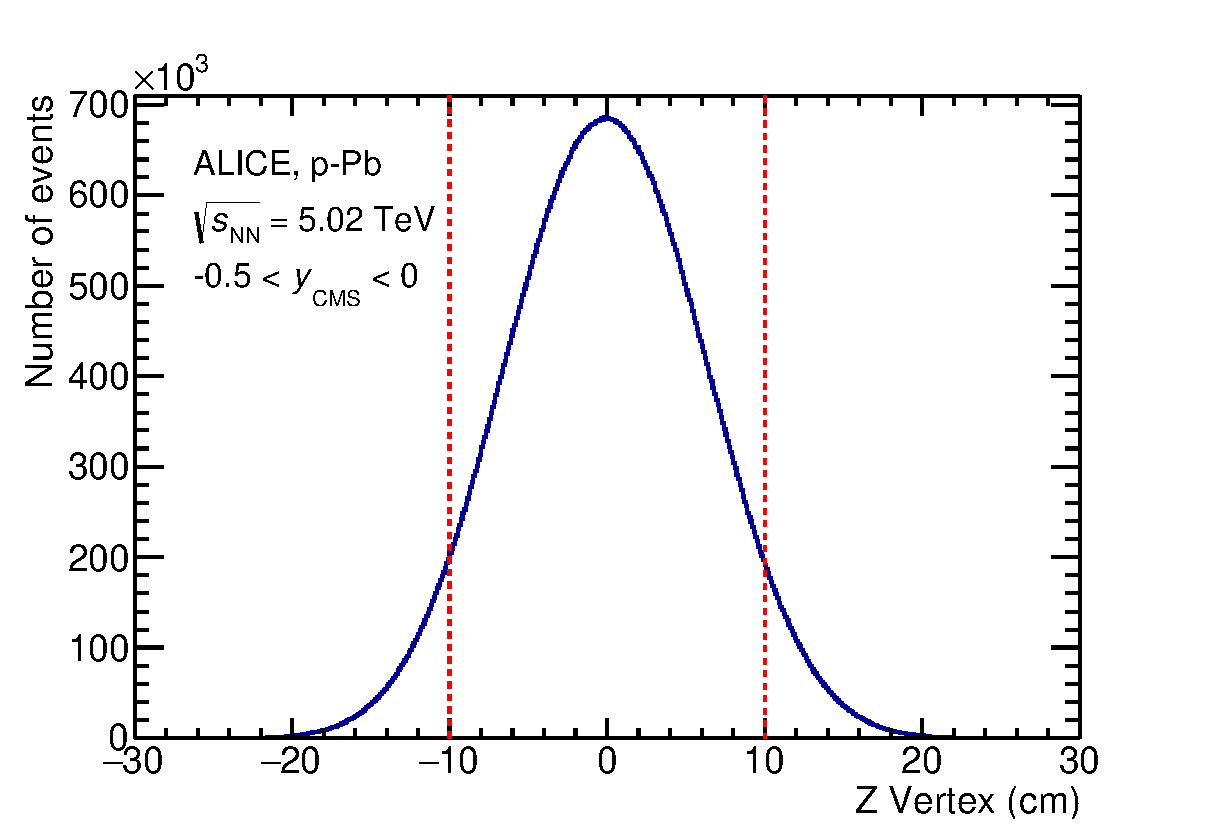
\includegraphics[width=7.cm]{./Version1/FigChapter5/Selection/pPbVertexZ.eps}
\hspace{0.5cm}
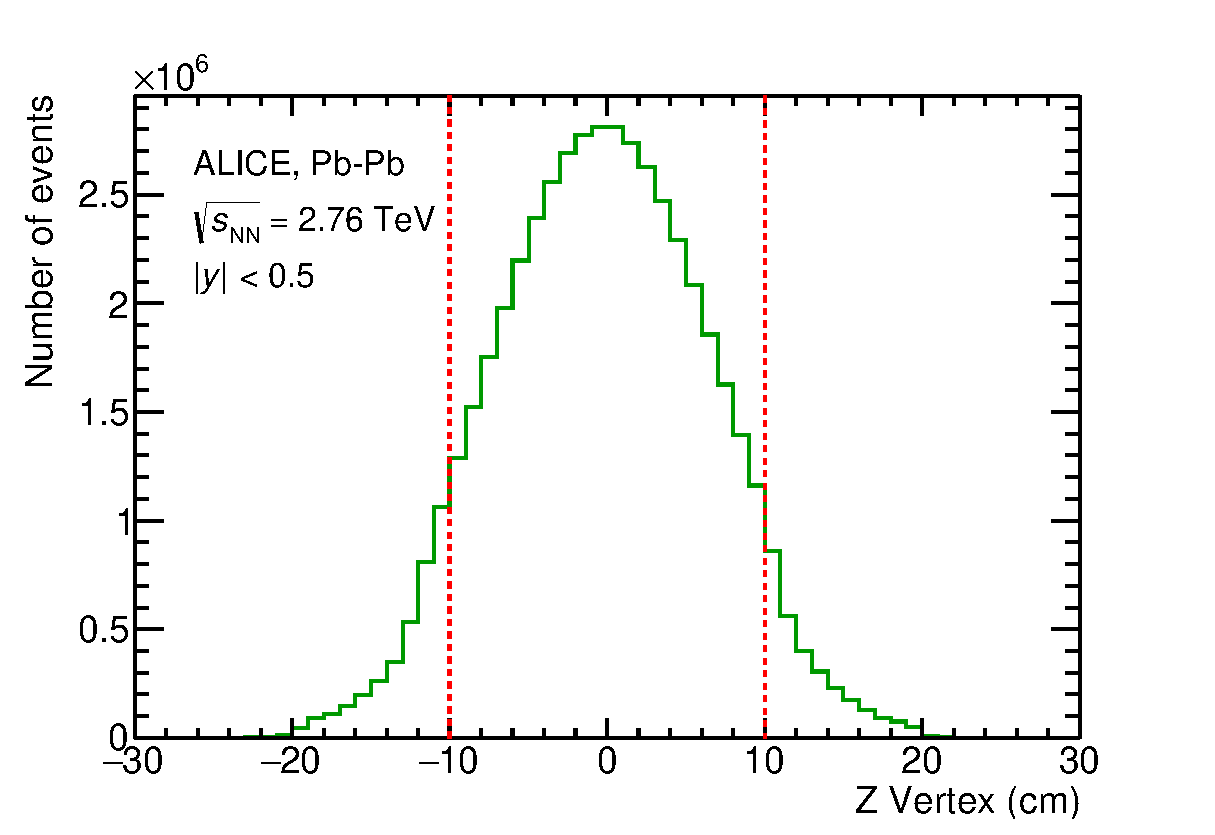
\includegraphics[width=7.cm]{./Version1/FigChapter5/Selection/PbPbVertexZ.eps}
\caption{Vertex-z coordinate distribution of the accepted events in p--Pb collision(Left) and in Pb--Pb collisions(Right). The red dashed line indicates vertex cut }
\label{fig:VzDistribution}
\end{center}
\end{figure}

%\begin{table}[htp]
%\begin{center}
%\begin{tabular}{|c|c|c|c|}
%\hline
%Event selection stage & number of events & percentage\\
%\hline
%\hline
%Original number of events &111.1 $\times$ 10 $^{6}$ &100.0\% \\
%\hline
%Number of triggered events (kINT7) &109.3 $\times$ 10 $^{6}$ &98.4\% \\
%\hline
%Events after PV position cut ($|$Vz$|$ $<$ 10 cm) & 97.5 $\times$ 10 $^{6}$ &87.8\% \\
%\hline
%Events after reject pile-up& 94.5 $\times$ 10 $^{6}$& 85.1\%\\
%\hline
%Events after number of SPD cluster cut ($\geq 1$)& 93.9 $\times$ 10 $^{6}$ &84.5\% \\
%\hline
%\end{tabular}
%\caption{Number of events at different selection stages.}\label{table:NEvent}
%\end{center}
%\end{table}






 Fig. \ref{fig:pPb:Centrality} shows the multiplicity distribution of the accepted events in p--Pb collision divided in bins of percentile. The each color on the histogram indicate the multiplicity ranges used in this analysis. Corresponding events for each multiplicity range are in Table \ref{table:NCentralityEvent}. 
 

\begin{figure}[htbp]
\begin{center}
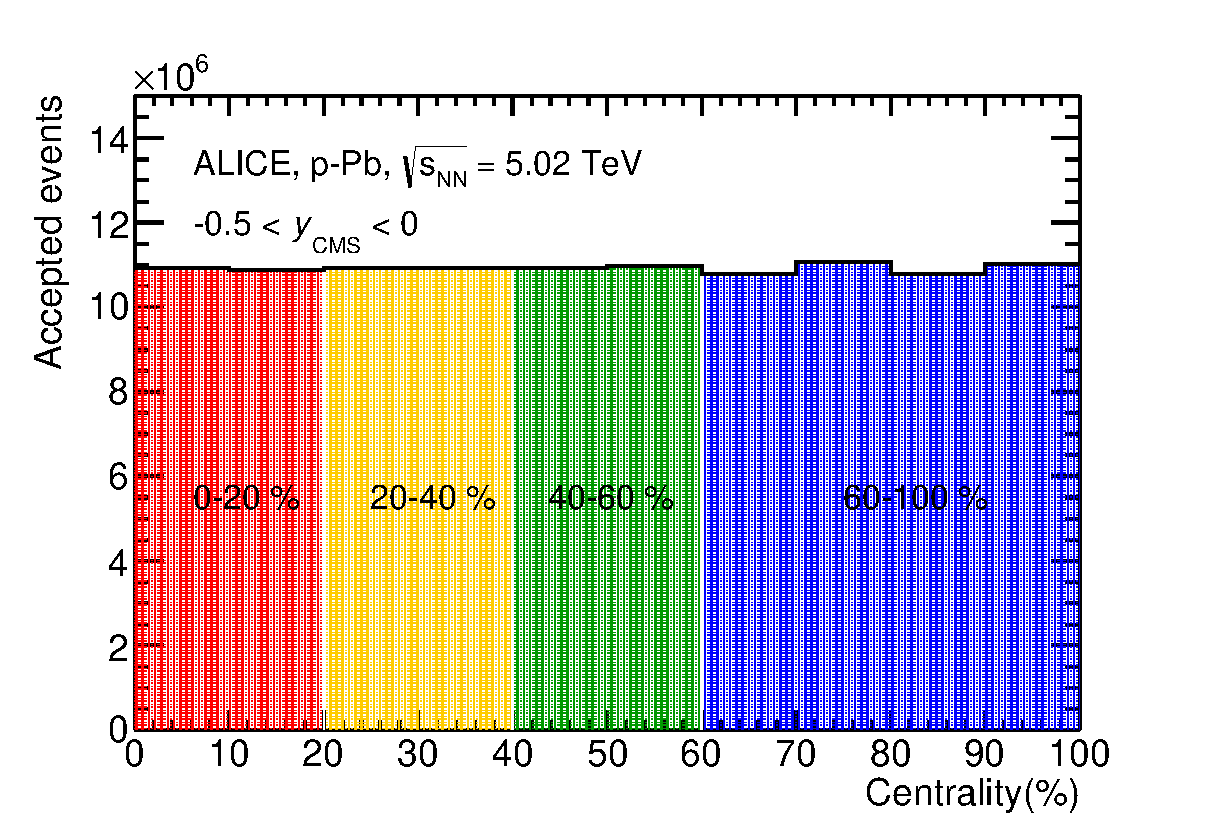
\includegraphics[width=10.cm]{./Version1/FigChapter5/Selection/pPbCentrality.eps}
\caption{ Multiplicity distribution of accepted events in p--Pb collision in percentile. The each color and labels define the four intervals in which the analysis in performed.}
\label{fig:pPb:Centrality}
\end{center}
\end{figure}

The distribution of centrality in each trigger used to select the events in Pb--Pb collision is shown in Fig. \ref{fig:PbPb:Centrality} and the reason why the centrality has step structure is that there are three different trigger classes classified by the amplitude threshold on VZERO detector.
Because the distribution of events as function of centrality is not a flat, this may lead to additional bias, in particular when one needs to combine the results from different triggers. For example, events from 40-80\% centrality bin have bias with high statistics in 40-60\%. In order to avoid this effect, we have applied a flattening procedure to have flat distribution of events as function of centrality. 
A brief explanation of the method is below : 

\begin{enumerate}
\item Histograms are obtained for the effective mass distribution in 1\% centrality bins and for the centrality distribution
\item The effective mass distributions are scaled in each 1\% centrality bin by a factor: \\
Factor = N{\footnotesize event in 20-40\%} / 20 / N{\footnotesize event in current 1\% bin}
\item Each bin in the centrality distribution is scaled using the factor described above
\item Histograms are added for centrality bins of interest: 0-10\%, 10-40\%, 40-80\%, 0-80\%
\end{enumerate}

The resulting number of events in each centrality classes is summarized in Table \ref{table:NCentralityEvent}.

\begin{figure}[htbp]
\begin{center}
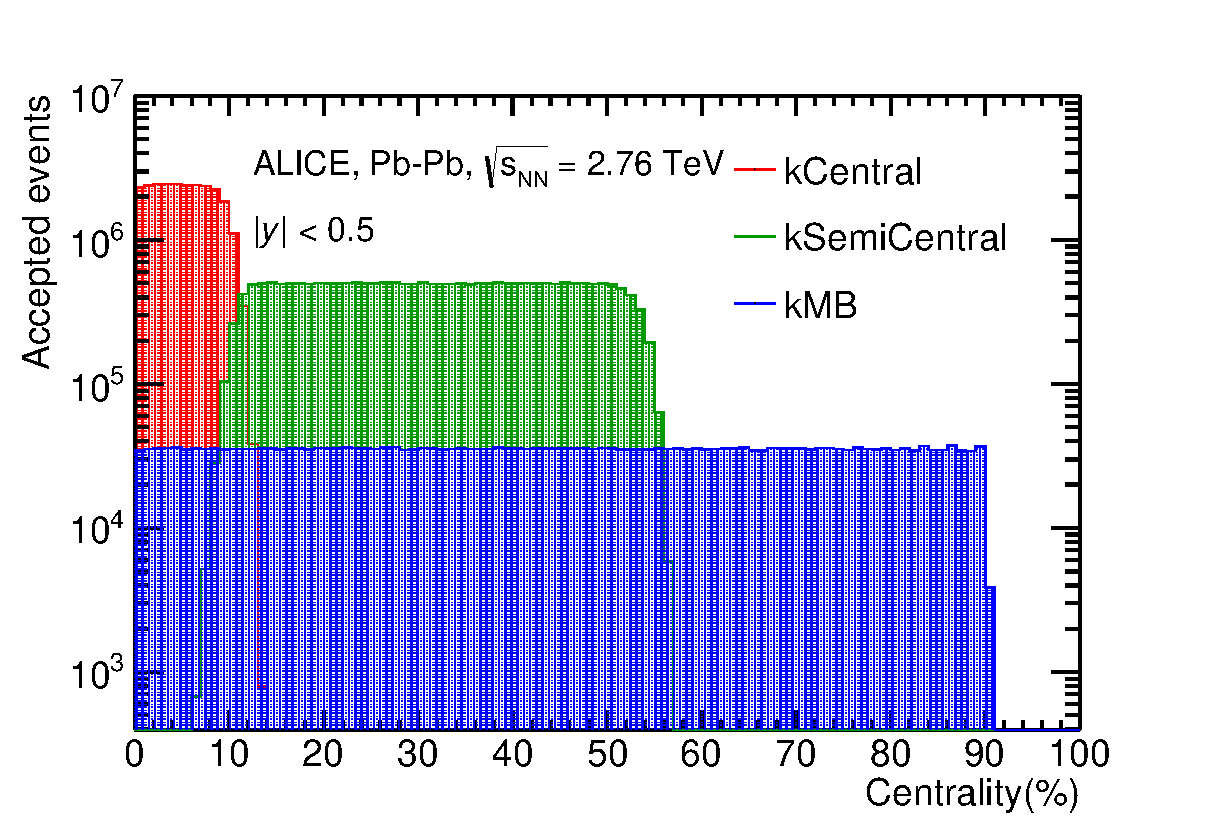
\includegraphics[width=10.cm]{./Version1/FigChapter5/Selection/PbPbCentrality.eps}
\caption{ Centrality distribution of three different trigger classes.}
\label{fig:PbPb:Centrality}
\end{center}
\end{figure}


\begin{table}[h!]
\centering
\begin{tabular}{lll}
\hline

p--Pb &   0-20\% &21.82 $\times$ 10 $^{6}$ \\
& 20-40\% &21.86 $\times$ 10 $^{6}$\\
& 40-60\% &21.91 $\times$ 10 $^{6}$ \\
& 60-100\% &43.68 $\times$ 10 $^{6}$ \\

\hline \noalign{\smallskip}

Pb--Pb& 0-10\%   & 5.58 $\times$ 10 $^{6}$ \\
& 10-40\%    & 16.73 $\times$ 10 $^{6}$ \\
& 40-80\% & 22.31 $\times$ 10 $^{6}$ \\
\hline\noalign{\smallskip}
\noalign{\smallskip}
\end{tabular}
\caption{Number of accepted and analyzed events per multiplicity/centrality interval}\label{table:NCentralityEvent}
\end{table}


\newpage
\subsubsection{Track and topological selection}\label{sec:Cut}

In comparison with the $\Xi^{*0}$ analysis carried out in pp collisions 
at $\sqrt{s}$ = 7 TeV~\cite{cite:Xi_pp}, track and topological selections were revised 
and adapted to the p--Pb dataset. Pions from strong decays of $\Xi^{*0}$ were selected
according to the criteria for primary tracks. As summarized in Table~\ref{tab:primary_selections}, 
all charged tracks were selected with \pt $>$ 0.15~ \gmom~ and $|\eta_{\mathrm{lab}}| <0.8$, as 
described in Ref.~\cite{cite:ALICEPerformance}. The primary tracks were chosen with the Distance of 
Closest Approach (DCA) to PV of less than 2 cm along the longitudinal direction (DCA$_z$)  and lower 
than 7$\sigma_r$ in the transverse plane (DCA$_r$), where $\sigma_r$ is the resolution of DCA$_r$. The 
$\sigma_r$ is strongly \pt-dependent and lower than 100 $\mu$m for 
$\pt >$~0.5~\gmom~\cite{cite:ALICEPerformance}. To ensure a good track reconstruction quality, 
candidate tracks were required to have at least one hit in one of the two innermost layers (SPD) of 
the ITS and to have at least 70 reconstructed points in the Time Projection Chamber (TPC), out of a 
maximum of 159. The Particle IDentification (PID) criteria for all decay daughters are based on the requirement 
that the specific energy loss (d$E$/d$x$) is measured in the TPC within three standard deviations 
($\sigma_\mathrm{TPC}$) from the expected value (d$E$/d$x_{\rm{exp}}$), computed using a Bethe-Bloch 
parametrization~\cite{cite:ALICEPerformance}.
\begin{table}[h!]
\centering
\begin{tabular}{lll}
\hline

Common track &  $|\eta_{\mathrm{lab}}|$ & $<0.8$ \\
 selections & \pt & $> 0.15$ GeV/$c$ \\
& PID $|$(d$E/$d$x)-$(d$E/$d$x)_{\rm{exp}}|$ & $<3$~$\sigma_{\rm{TPC}}$ \\
\hline \noalign{\smallskip}

Primary track& DCA$_z$ to PV         & $<2$ cm \\
 selections & DCA$_r$ to PV         & $<7\sigma_r$-10$\sigma_r$ (\pt) \\
& number of SPD points & $\geq 1$ \\
& number of TPC points & $>70$ \\
& $\chi^{2}$ per cluster & $<4$ \\
\hline\noalign{\smallskip}
\noalign{\smallskip}
\end{tabular}
\caption{Track selections common to all decay daughters and primary track selections applied 
to the charged pions from decays of $\Xi^{*0}$.}  
\label{tab:primary_selections}     \end{table}


\begin{figure}[htbp]
\begin{center}
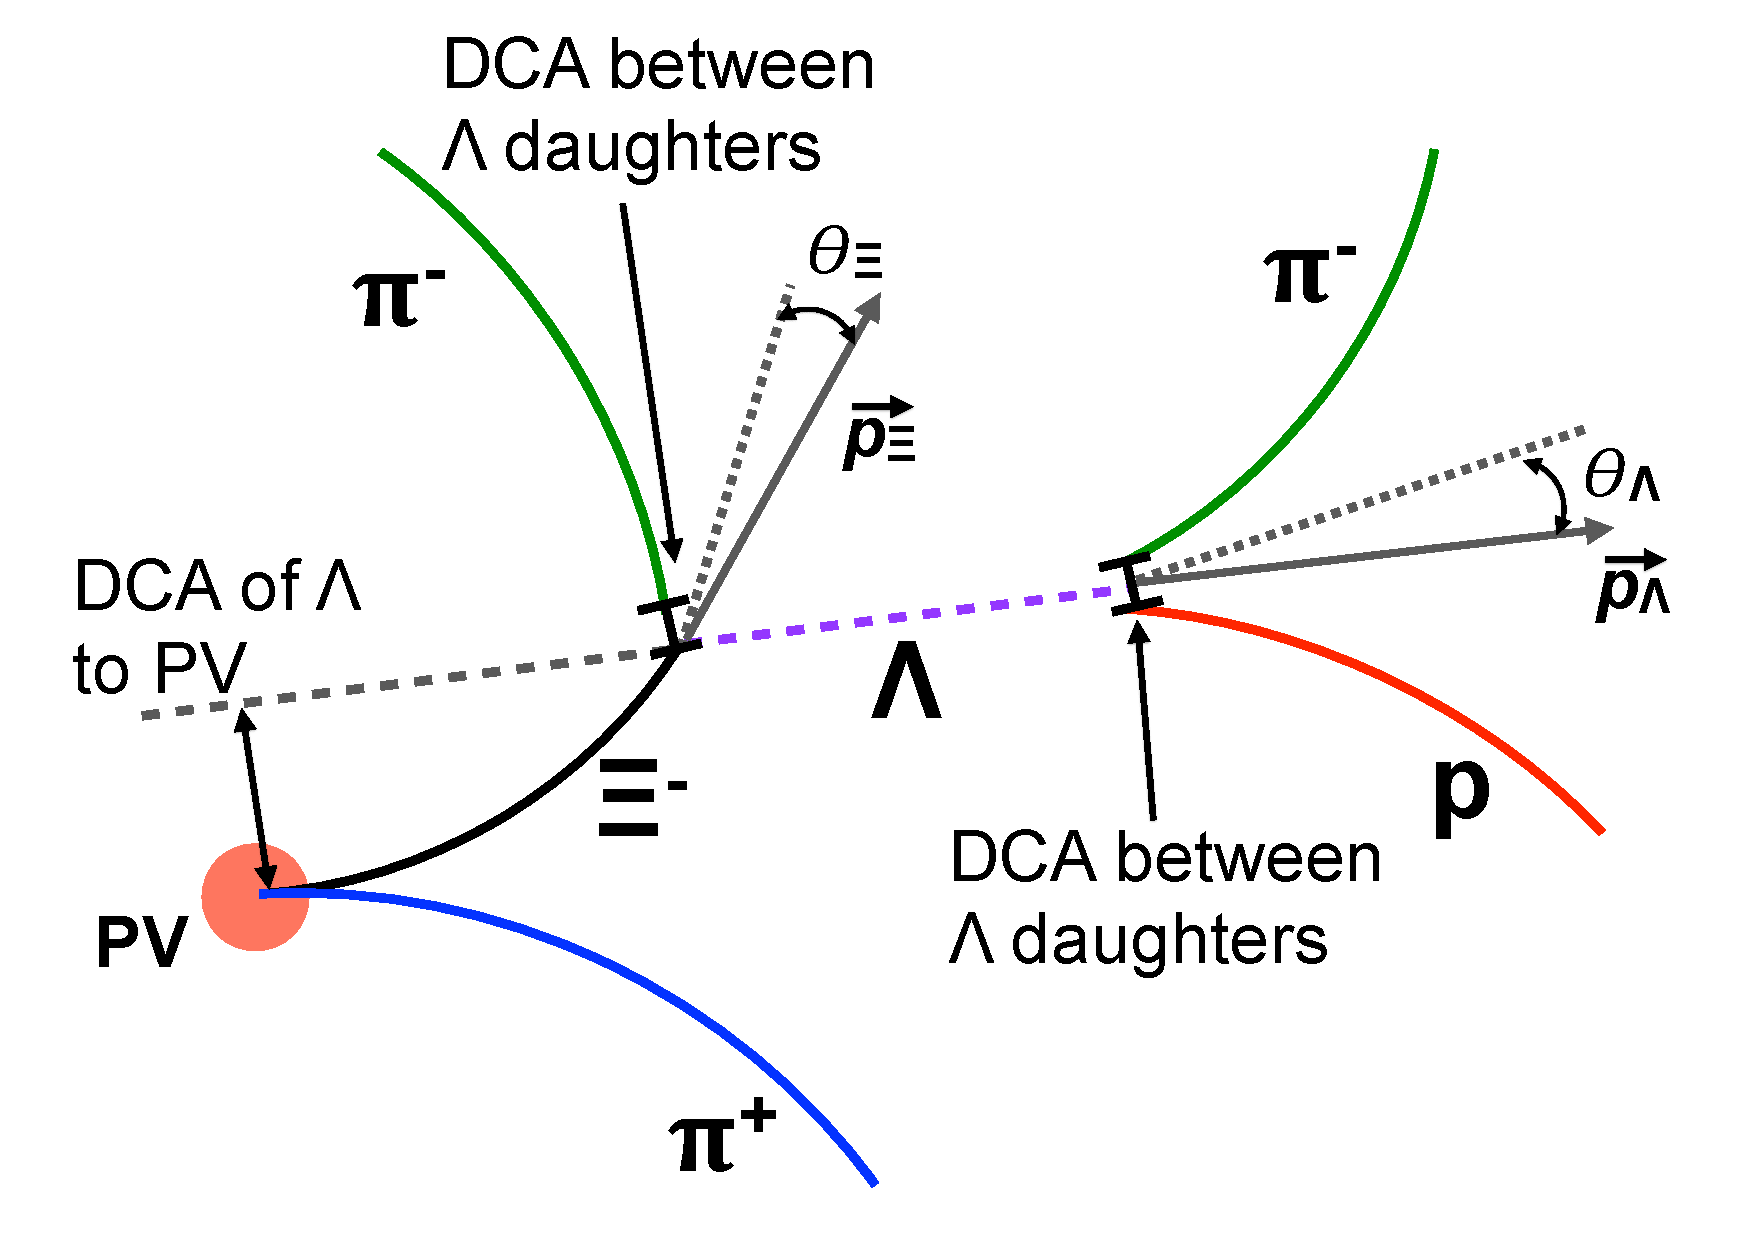
\includegraphics[width=11.cm]{./Version1/FigChapter5/Selection/Sketch.pdf}
\caption{ Sketch of the decay modes for $\Xi^{*0}$ and depiction of the track and topological selection criteria.}
\label{fig:decay}
\end{center}
\end{figure}

Since pions and protons from weak decay of $\Lambda$ ($ \cL \tau = 7.89$ cm~\cite{cite:PDG}) and 
pions from weak decay of $\Xi^{-}$ ($ \cL \tau = 4.91$ cm~\cite{cite:PDG}) are produced away from the PV, 
specific topological and track selection criteria, as summarized in Table~\ref{tab:selections}, were 
applied~\cite{ cite:Xi_pPb,cite:Xi_pp,cite:lambda_pp}.



\begin{table}[h!]
\centering
\begin{tabular}{lll}
\hline\noalign{\smallskip}
Topological cuts & p--Pb & Pb--Pb\\
\hline
DCA$_r$ of $\Lambda$ decay products to PV   & $>0.06$ cm& $>0.11$ cm \\
DCA between $\Lambda$ decay products   & $<1.4$cm & $<0.95$ cm\\
DCA of $\Lambda$ to PV                   & $>0.015$  cm& $>0.06$ \\
cos$\theta_\Lambda$ & $>0.875$  &          $>0.998$ \\
$r(\Lambda)$          & 0.2 $<r(\Lambda)<$ 100 cm   &  0.2 $<r(\Lambda)<$ 100 cm    \\
$|M_{p\pi} - m_\Lambda|$        & $<$ 7 \mmass  &$<$ 7 \mmass\\
DCA$_r$ of pion (from $\Xi^{-}$) to PV     & $>0.015$ cm &$>0.035$ cm\\
DCA between $\Xi^{-}$ decay products  & $<1.9$ cm&$<0.275$\\
cos$\theta_\Xi$     & $>0.981$    & $>0.9992$\\
$r(\Xi^-)$            & 0.2 $<r(\Xi^-)<$ 100 cm      &  0.2 $<r(\Xi^-)<$ 100 cm  \\
$|M_{\Lambda\pi} - m_\Xi|$        &  $<$ 7 \mmass  &   $<$ 7 \mmass   \\
\hline
\end{tabular}
\caption{Topological and track selection criteria.}
\label{tab:selections}. 
\end{table}

In the analysis of $\Xi^{*0}$, $\Lambda$ and $\pi$ from $\Xi^{-}$ were 
selected with a DCA of less than 1.9~cm and with a DCA$_r$ to the PV greater than 0.015 cm. 
The $\Lambda$ daughter particles ($\pi$ and p) were required to have a DCA$_r$ to the PV greater 
than 0.06 cm, while the DCA between the two particles was required to be less than 1.4 cm. Cuts on 
the invariant mass, the cosine of the pointing angle ($\theta_\Lambda$, $\theta_\Xi$) and the radius of 
the fiducial volume ($r(\Lambda)$, $r(\Xi)$) in Table~\ref{tab:selections} were applied to optimize 
the balance of purity and efficiency of each particle sample. 


\newpage
\subsubsection{Particle identification}\label{sec:pPb:PID}
PID selection criteria are applied for
 
 \begin{enumerate}
\item $\pi^{\pm}$ (last emitted $\pi$) and proton from $\Lambda$
\item $\pi^{\pm}$ (second emitted $\pi$)   from $\Xi^{\pm}$
\item $\pi^{\pm}$ (first emitted $\pi$) from  $\Xi$(1530)$^{0}$
\end{enumerate}
 by using TPC. On TPC dE/dx versus momentum distribution, 3$\sigma$ cuts are applied to TPC for selecting each of the particles. The TPC $\mathrm{d}E/\mathrm{d}x$ selection allows to have better signal with $\sim$20\% increase of significance. 
  
 
\begin{figure}[htbp]
\begin{center}
\includegraphics[width=7.0cm]{./Version1/FigChapter5/Selection/pPbTPC3rdPion.eps}
\hspace{0.5cm}
\includegraphics[width=7.0cm]{./Version1/FigChapter5/Selection/pPbTPC3rdPionAfter.eps}
\label{fig:pPb:TPCpionFirstEmitted} 
\caption{ TPC $\mathrm{d}E/\mathrm{d}x$ as function of transverse momentum for total (top) and selected first emitted $\pi$ in 3$\sigma$ (bottom) }
\end{center}
\end{figure}

 
 \begin{figure}[htbp]
\begin{center}
\includegraphics[width=7.0cm]{./Version1/FigChapter5/Selection/pPbTPC2ndPion.eps}
\hspace{0.5cm}
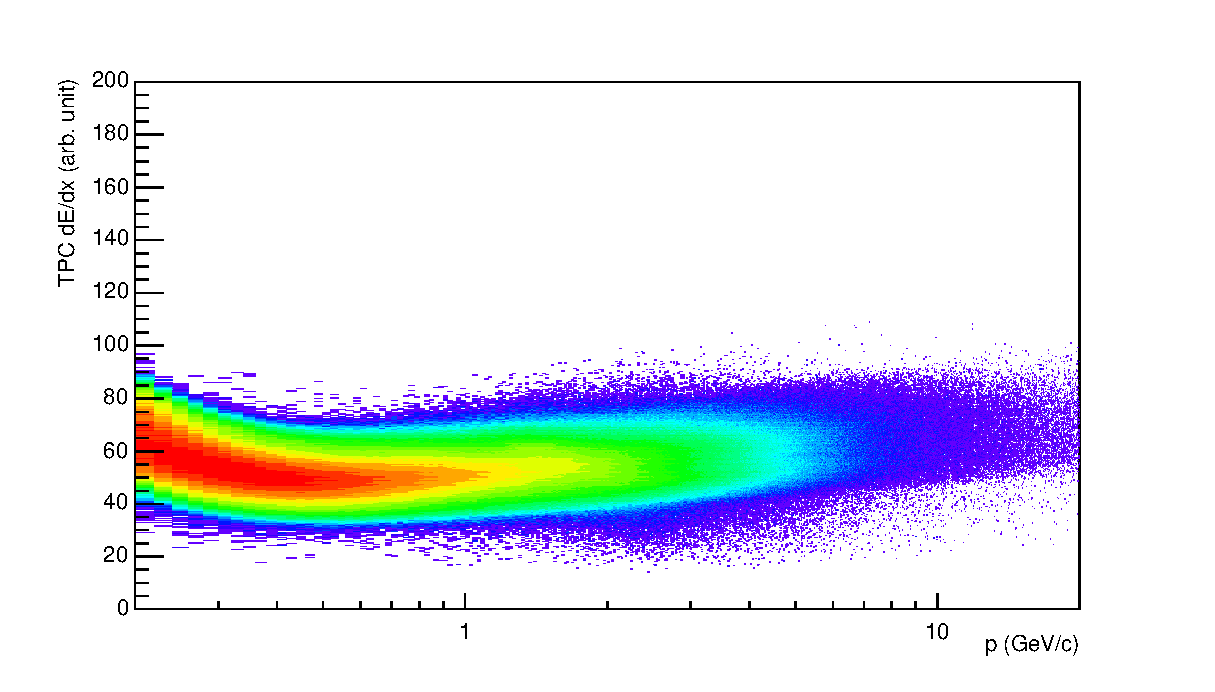
\includegraphics[width=7.0cm]{./Version1/FigChapter5/Selection/pPbTPC2ndPionAfter.eps}
\label{fig:pPb:TPCpionSecondEmitted} 
\caption{ TPC $\mathrm{d}E/\mathrm{d}x$ as function of transverse momentum for total (top) and selected second emitted $\pi$ in 3$\sigma$(bottom) }
\end{center}
\end{figure}


\begin{figure}[htbp]
\begin{center}
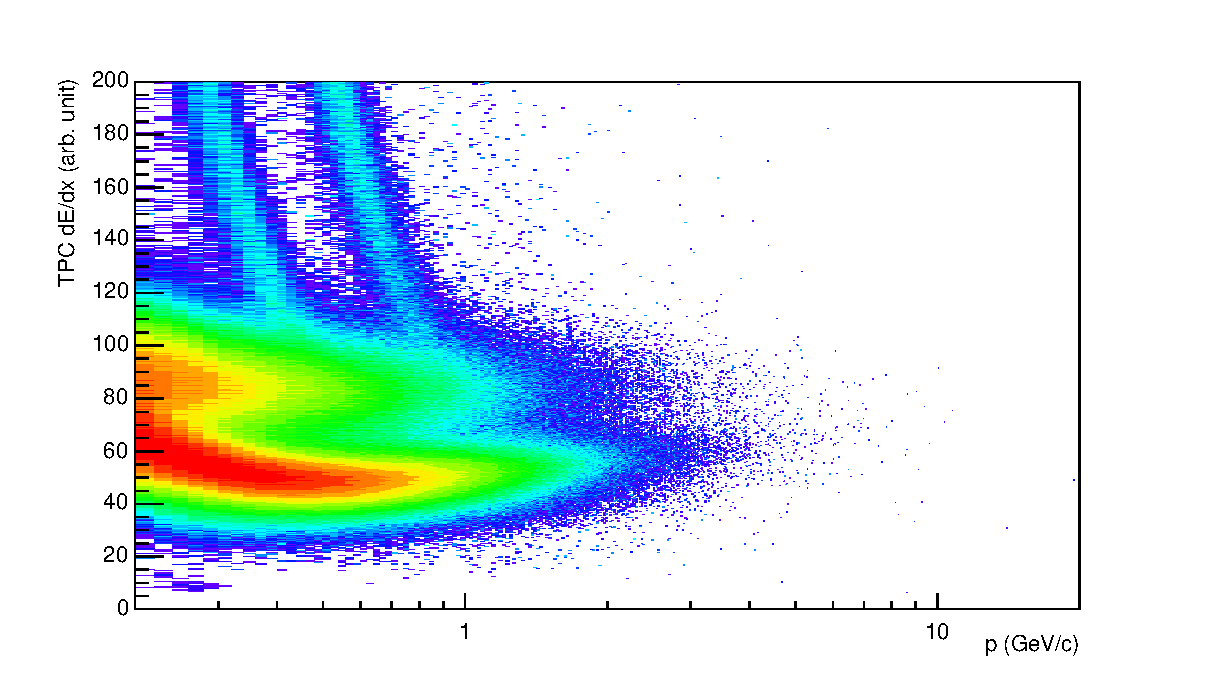
\includegraphics[width=7.0cm]{./Version1/FigChapter5/Selection/pPbTPC1stPion.eps}
\hspace{0.5cm}
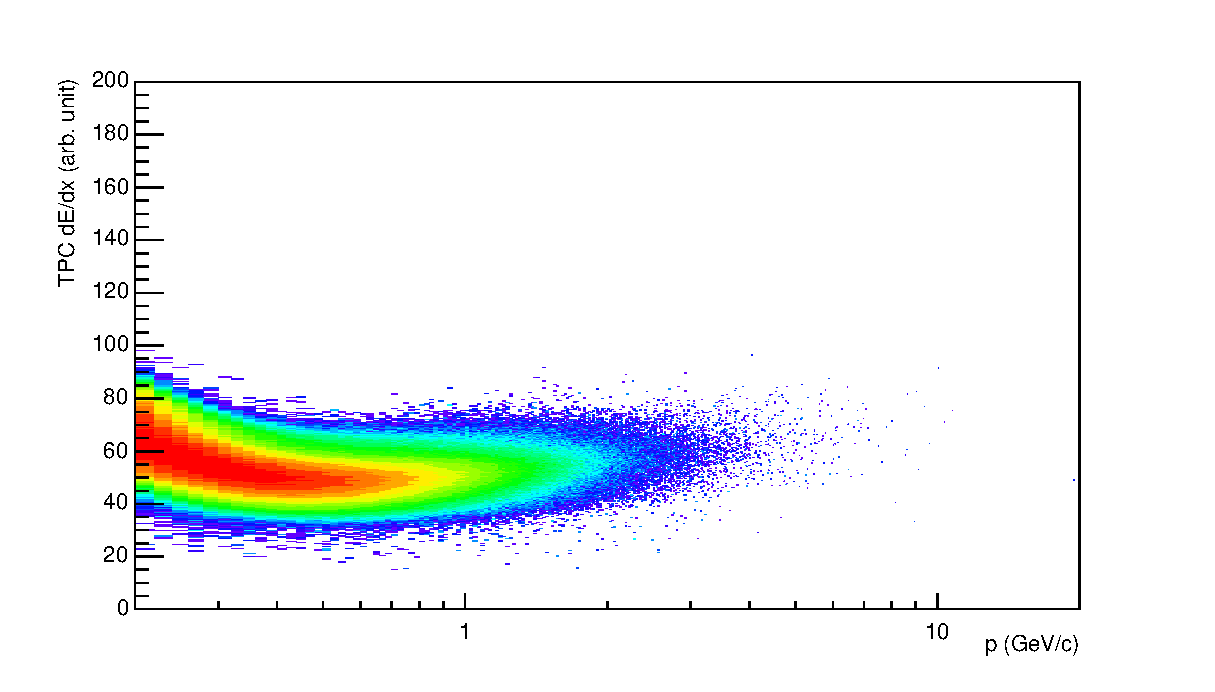
\includegraphics[width=7.0cm]{./Version1/FigChapter5/Selection/pPbTPC1stPionAfter.eps}
\label{fig:pPb:TPCpionLastEmitted} 
\caption{ TPC $\mathrm{d}E/\mathrm{d}x$ as function of transverse momentum for total (top) and selected last emitted $\pi$ in 3$\sigma$(bottom) }
\end{center}
\end{figure}


\begin{figure}[htbp]
\begin{center}
\includegraphics[width=7.0cm]{./Version1/FigChapter5/Selection/pPbTPCp.eps}
\hspace{0.5cm}
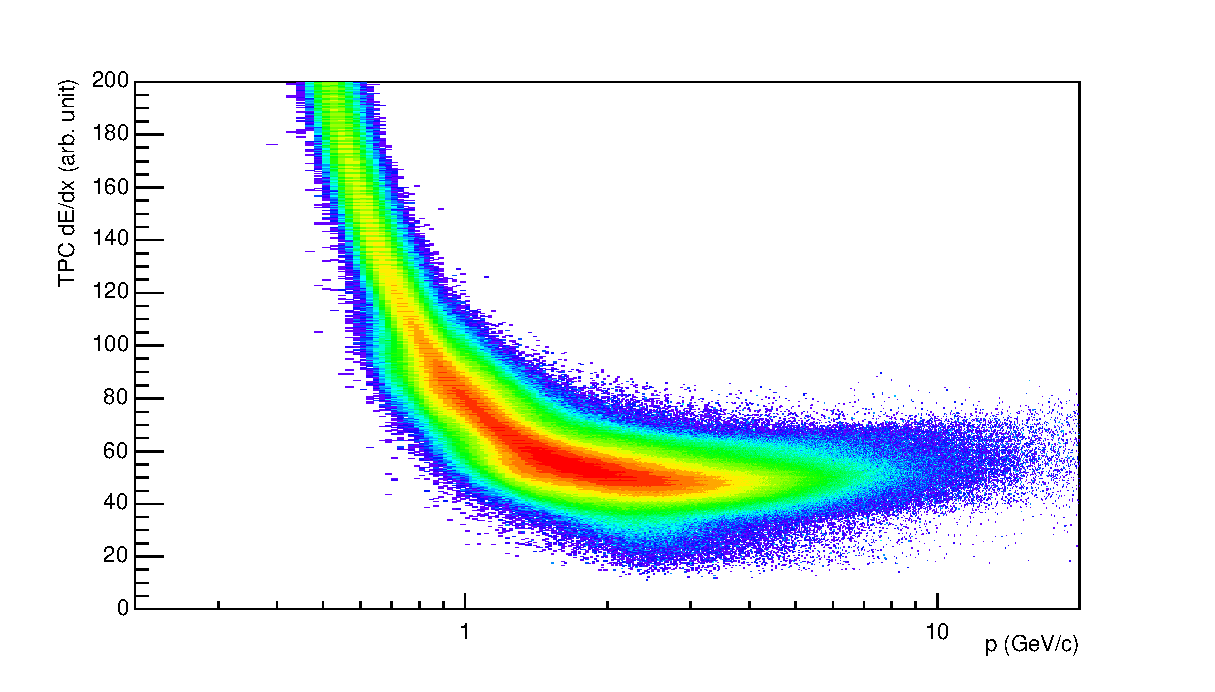
\includegraphics[width=7.0cm]{./Version1/FigChapter5/Selection/pPbTPCpAfter.eps}
\label{fig:pPb:TPCp} 
\caption{ TPC $\mathrm{d}E/\mathrm{d}x$ as function of transverse momentum for total (top) and selected proton in 3$\sigma$(bottom) }
\end{center}
\end{figure}

%%%
\begin{figure}[htbp]
\begin{center}
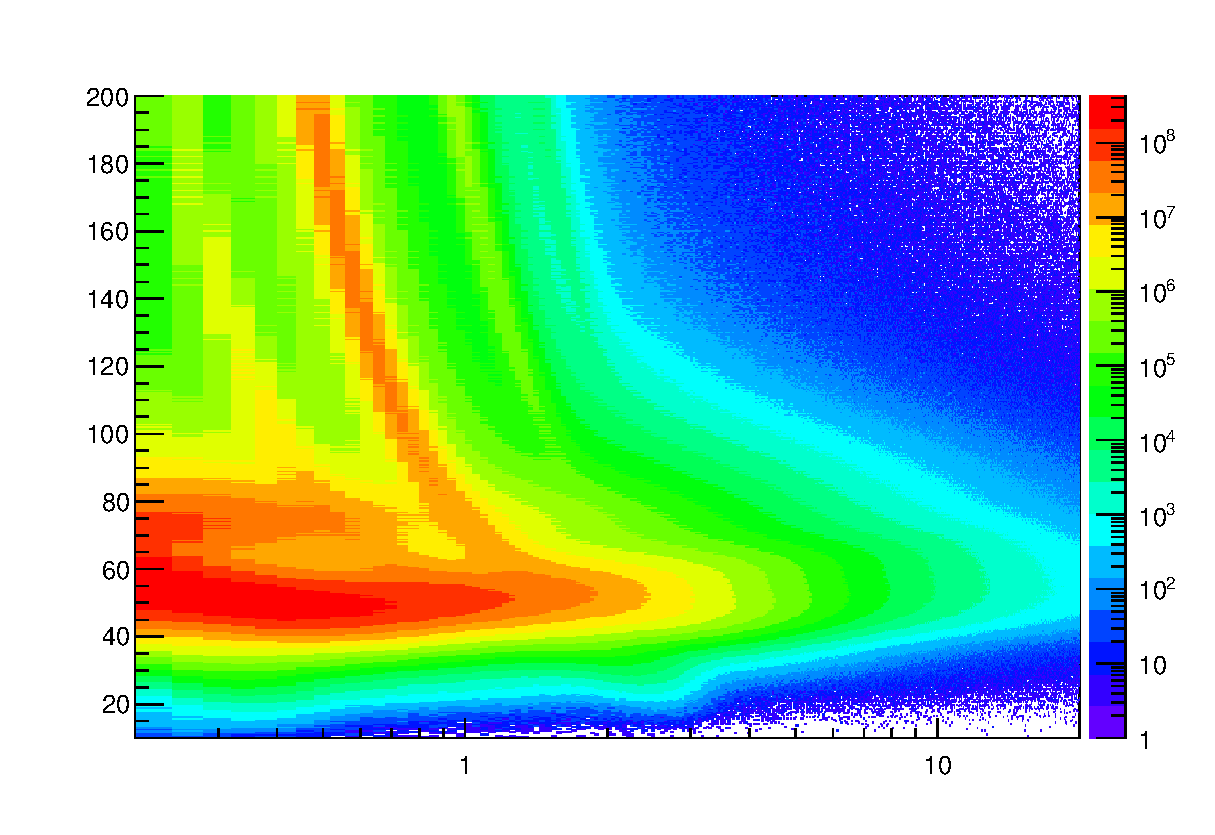
\includegraphics[width=7.0cm]{./Version1/FigChapter5/Selection/PbPbTPC3rdPion.eps}
\hspace{0.5cm}
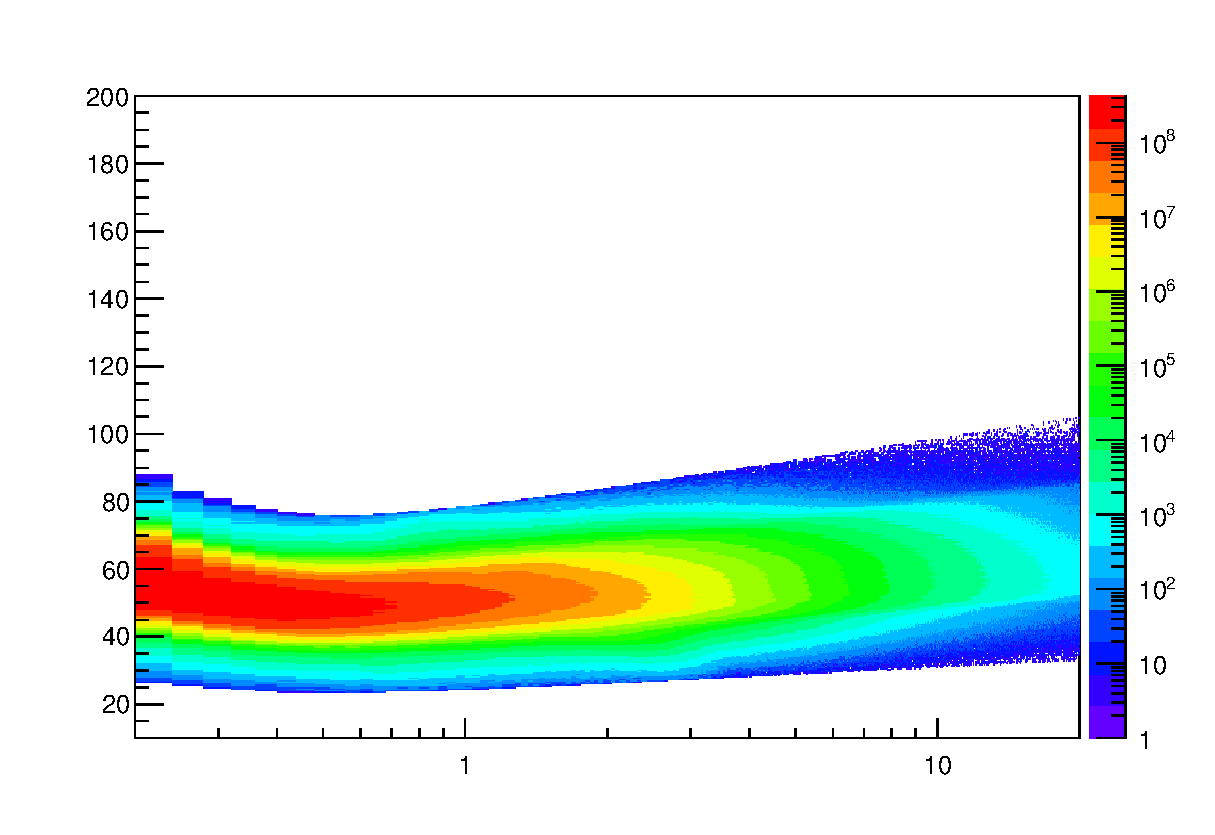
\includegraphics[width=7.0cm]{./Version1/FigChapter5/Selection/PbPbTPC3rdPionAfter.eps}
\label{fig:PbPb:TPCpionFirstEmitted} 
\caption{ TPC $\mathrm{d}E/\mathrm{d}x$ as function of transverse momentum for total (top) and selected first emitted $\pi$ in 3$\sigma$ (bottom) }
\end{center}
\end{figure}

 
 \begin{figure}[htbp]
\begin{center}
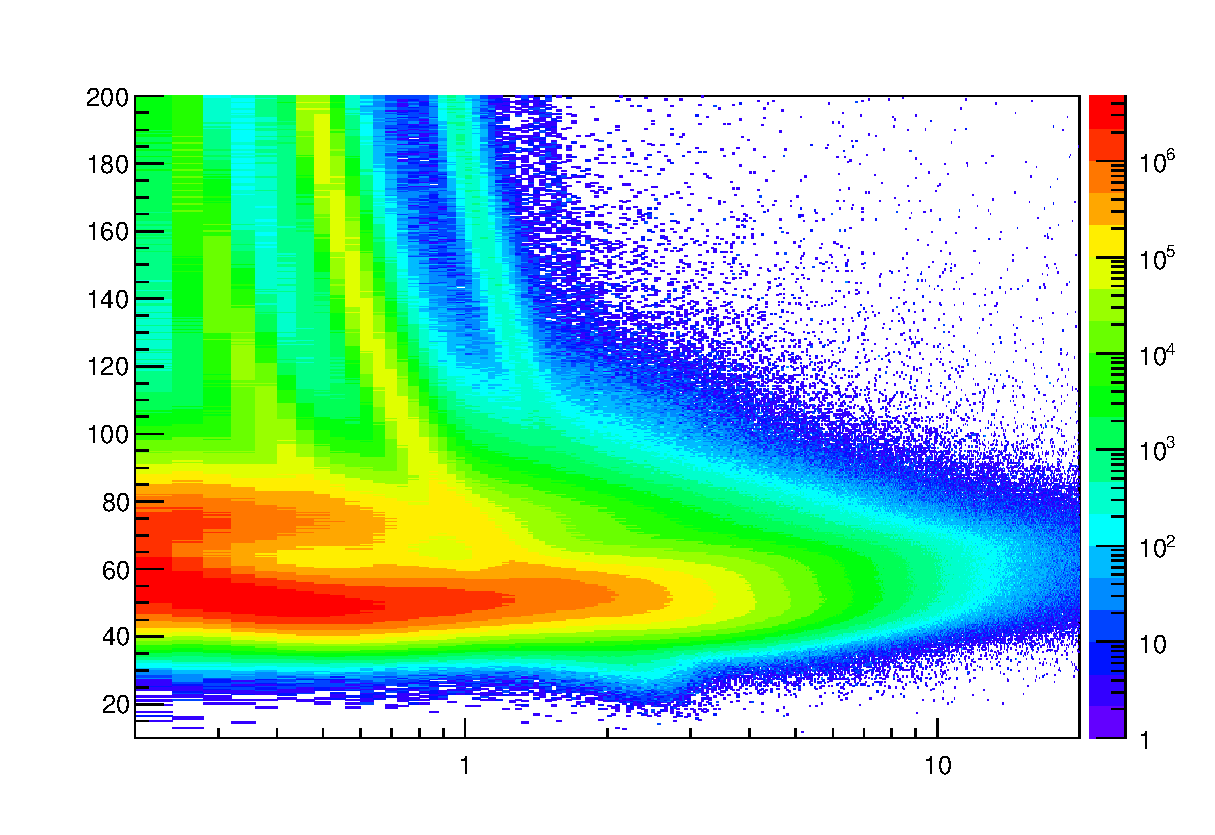
\includegraphics[width=7.0cm]{./Version1/FigChapter5/Selection/PbPbTPC2ndPion.eps}
\hspace{0.5cm}
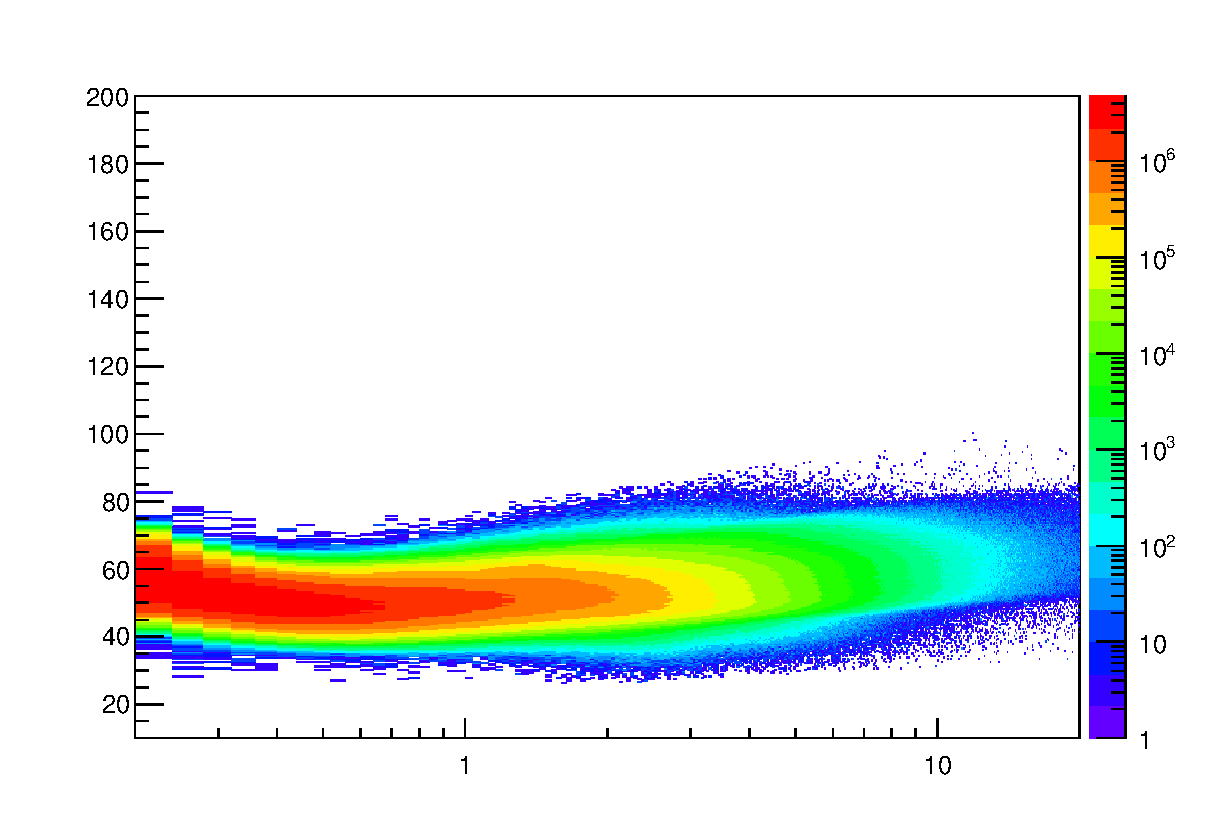
\includegraphics[width=7.0cm]{./Version1/FigChapter5/Selection/PbPbTPC2ndPionAfter.eps}
\label{fig:PbPb:TPCpionSecondEmitted} 
\caption{ TPC $\mathrm{d}E/\mathrm{d}x$ as function of transverse momentum for total (top) and selected second emitted $\pi$ in 3$\sigma$(bottom) }
\end{center}
\end{figure}


\begin{figure}[htbp]
\begin{center}
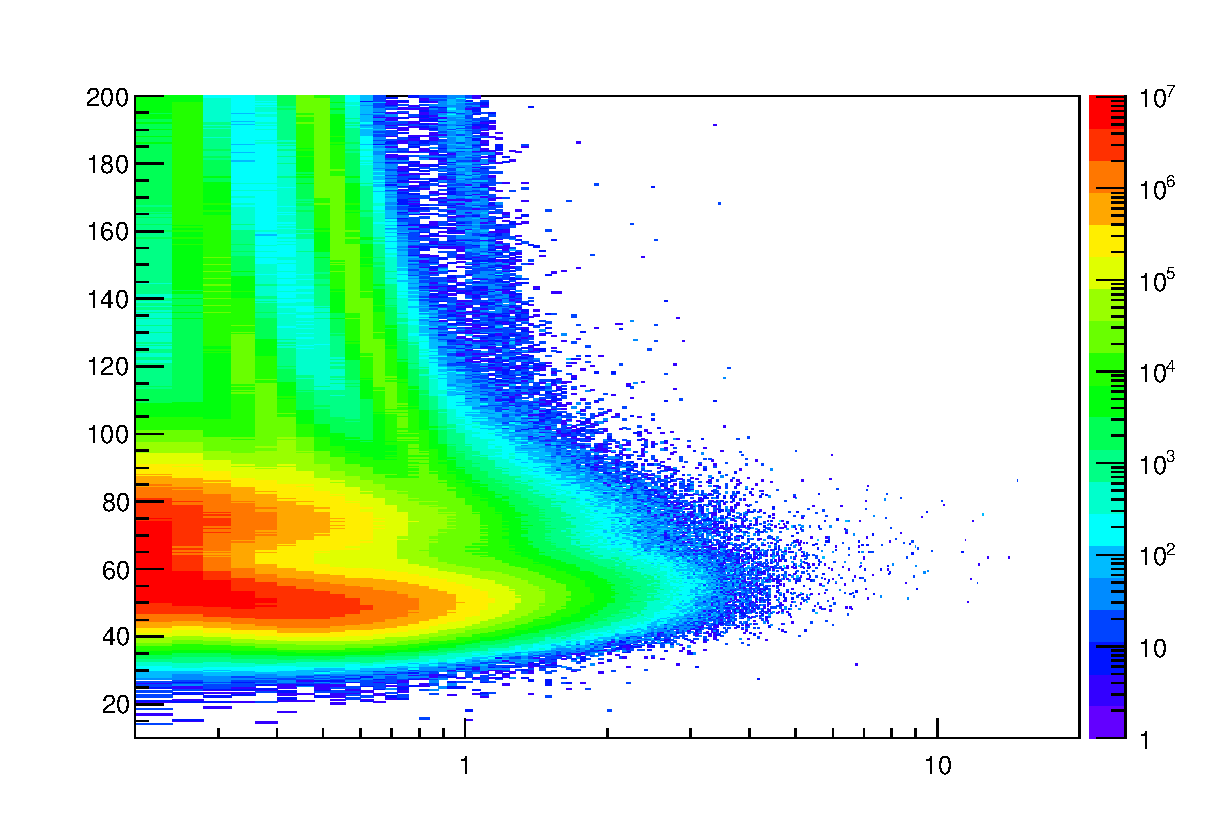
\includegraphics[width=7.0cm]{./Version1/FigChapter5/Selection/PbPbTPC1stPion.eps}
\hspace{0.5cm}
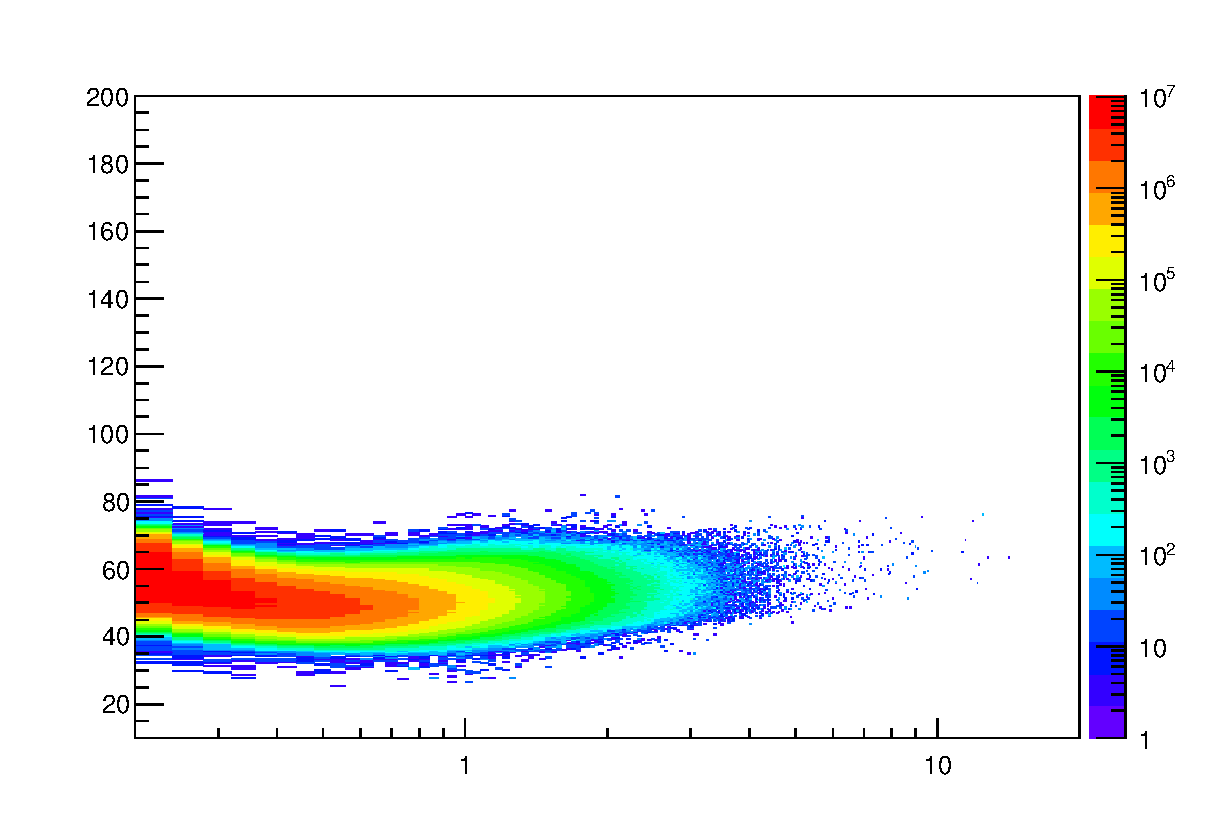
\includegraphics[width=7.0cm]{./Version1/FigChapter5/Selection/PbPbTPC1stPionAfter.eps}
\label{fig:PbPb:TPCpionLastEmitted} 
\caption{ TPC $\mathrm{d}E/\mathrm{d}x$ as function of transverse momentum for total (top) and selected last emitted $\pi$ in 3$\sigma$(bottom) }
\end{center}
\end{figure}


\begin{figure}[htbp]
\begin{center}
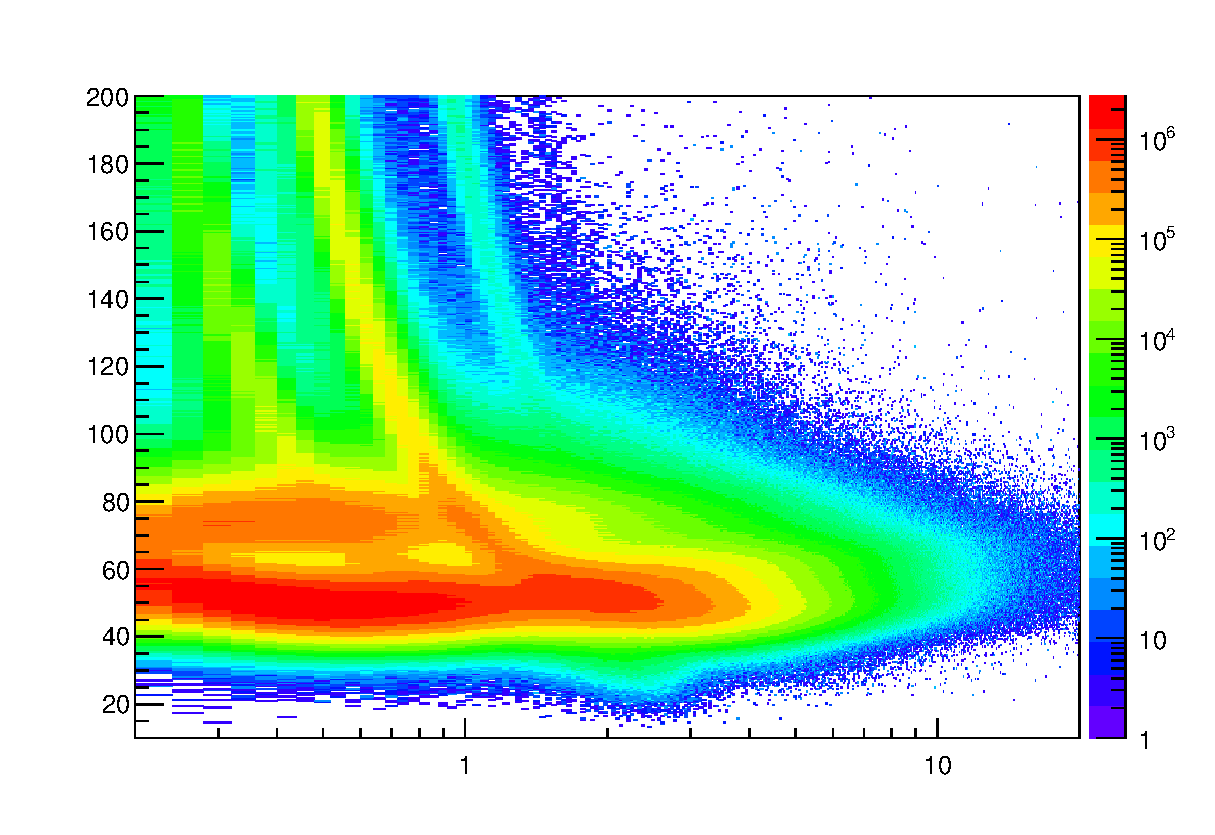
\includegraphics[width=7.0cm]{./Version1/FigChapter5/Selection/PbPbTPCp.eps}
\hspace{0.5cm}
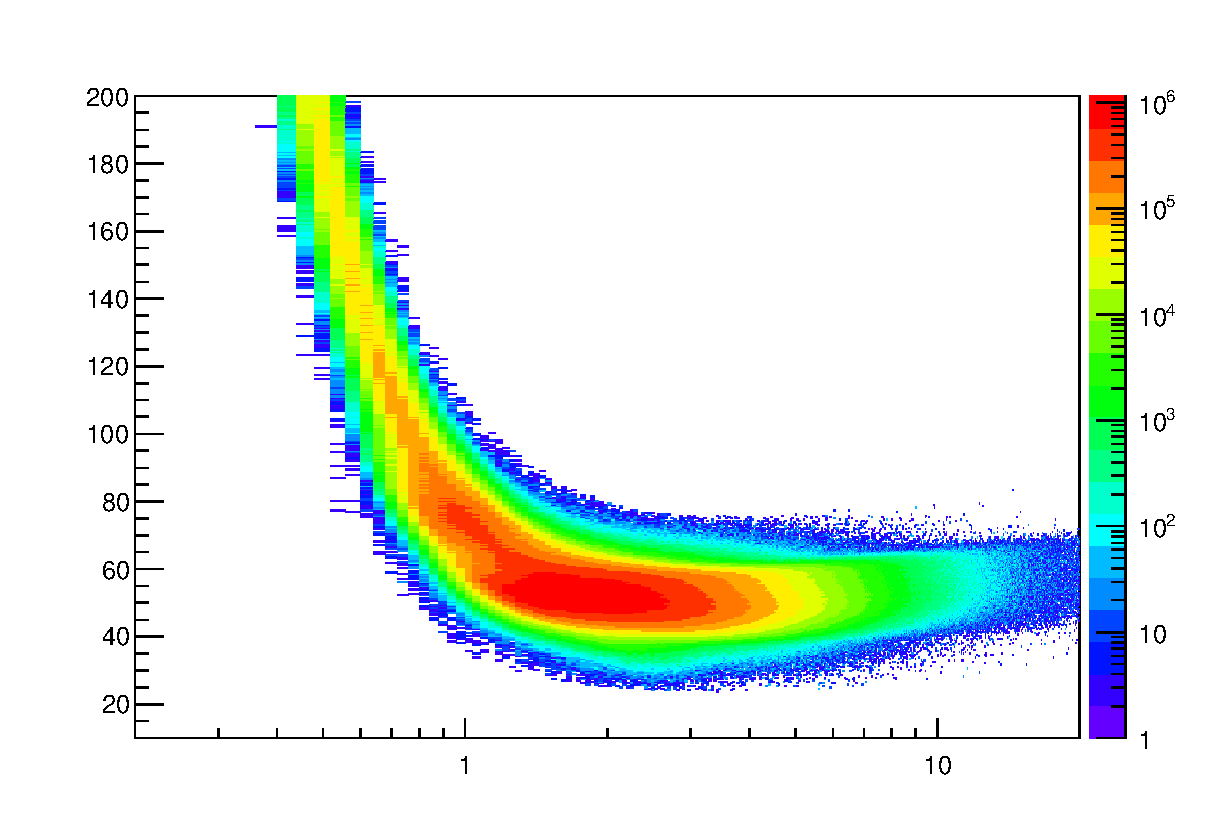
\includegraphics[width=7.0cm]{./Version1/FigChapter5/Selection/PbPbTPCpAfter.eps}
\label{fig:PbPb:TPCp} 
\caption{ TPC $\mathrm{d}E/\mathrm{d}x$ as function of transverse momentum for total (top) and selected proton in 3$\sigma$(bottom) }
\end{center}
\end{figure}



 
\newpage
\subsubsection{Signal extraction}\label{sec:pPb:signal}

The $\Xi^{*0}$ signals were reconstructed by invariant-mass analysis 
of candidates for the decay products in each transverse momentum interval of the resonance 
particle, and for each multiplicity class. The  $\Xi^-\pi^+$($\Xi^+\pi^-$) invariant mass distribution is reported in Figure \ref{fig:sigpPbb} for semi-central events (20-40\%) in p--Pb collisions and Figure \ref{fig:sigPbPbb} for central events(0-10\%) in Pb--Pb collisions.


\begin{figure}[htbp]
\begin{center}
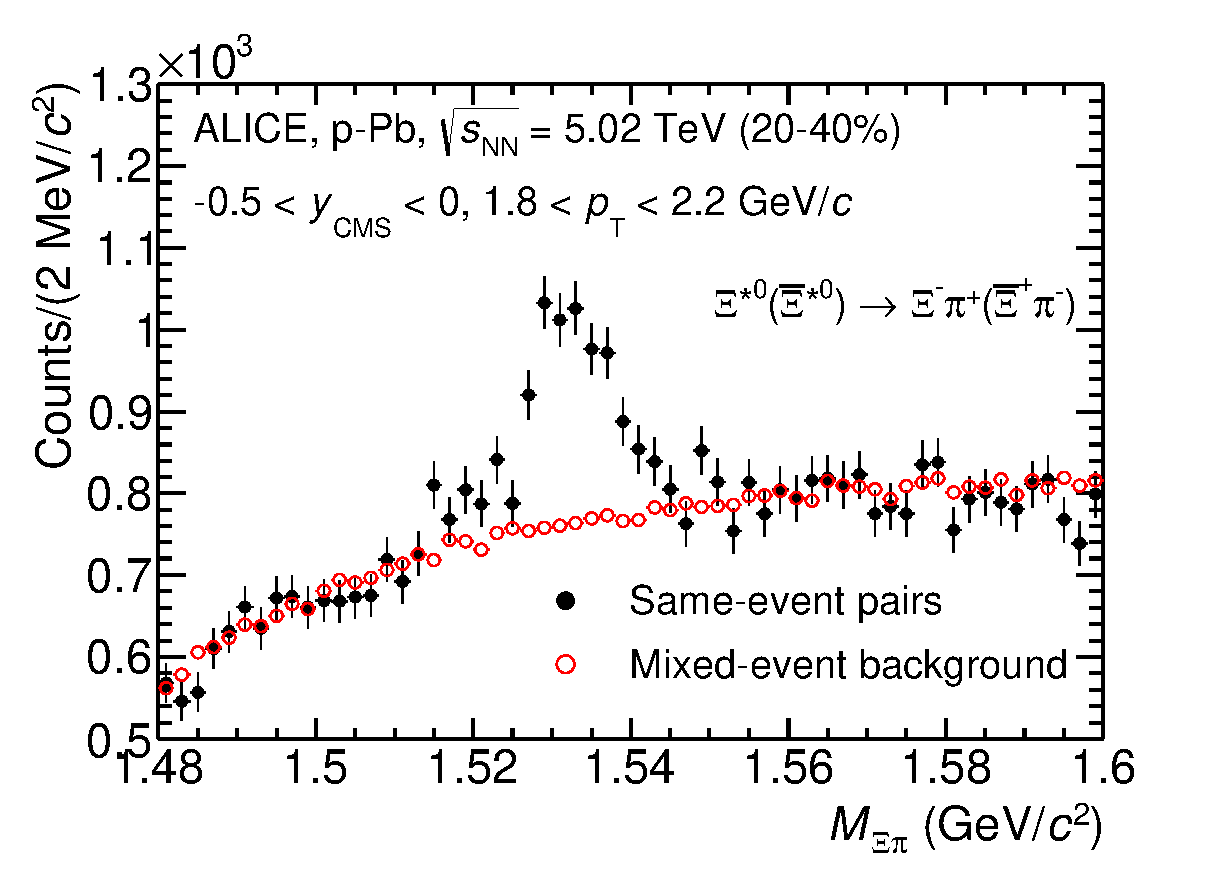
\includegraphics[width=12.0cm]{./Version1/FigChapter5/Extraction/SigpPb_Before.eps}
\hspace{0.5cm}
\label{fig:sigpPbb} 
\caption{ The $\Xi^{\mp}\pi^{\pm}$ invariant mass distribution (Same-event pairs) in 
1.8$<$ \pt $<$2.2~\gmom~and for the multiplicity class 20-40\%. The background shape, 
using pairs from different events (Mixed-event background), is normalised to the counts in 
1.49~$<$~$M_{\Xi\pi}$~$<$~1.51~\Gmass~and 1.56~$<$~$M_{\Xi\pi}$~$<$~1.58~\Gmass. }
\end{center}
\end{figure}

\begin{figure}[htbp]
\begin{center}
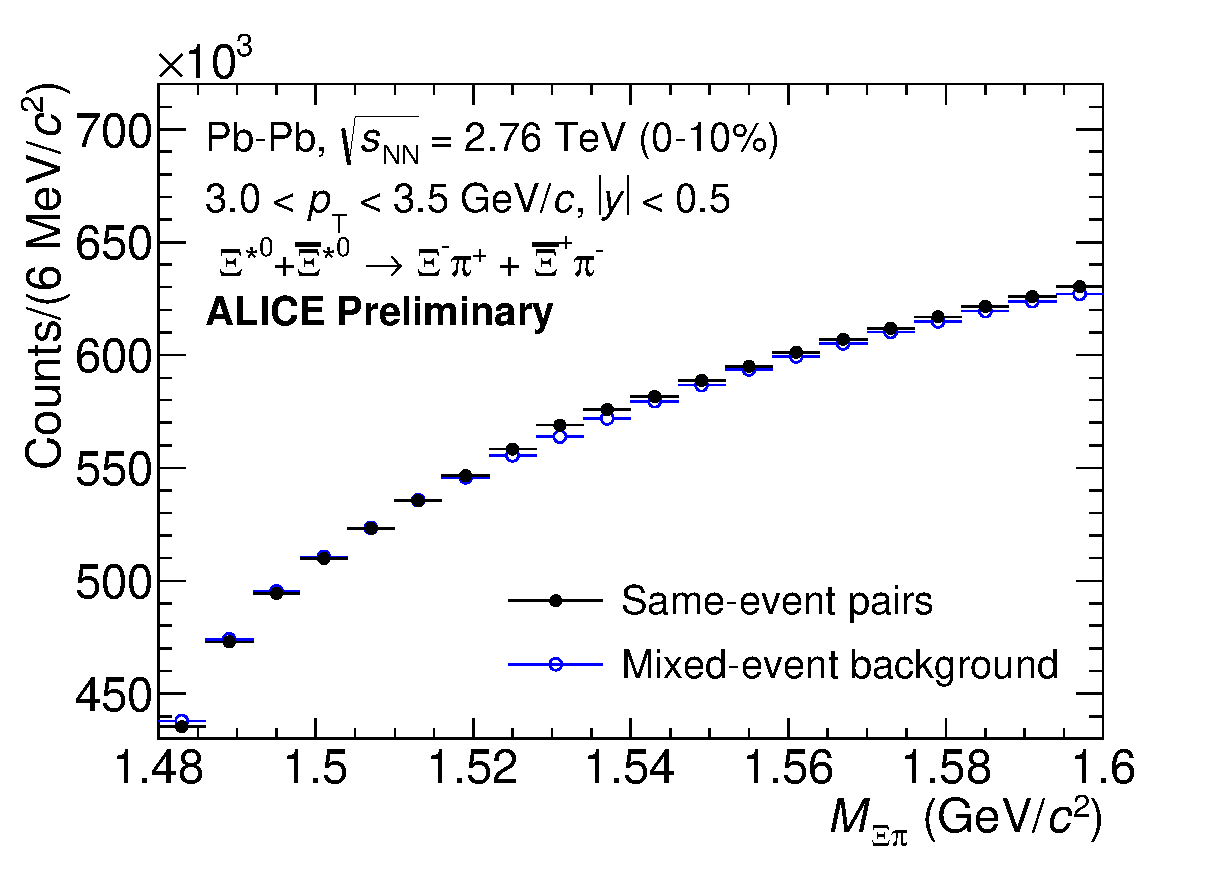
\includegraphics[width=12.0cm]{./Version1/FigChapter5/Extraction/SigPbPb_Before.eps}
\hspace{0.5cm}
\label{fig:sigPbPbb} 
\caption{ The $\Xi^{\mp}\pi^{\pm}$ invariant mass distribution (Same-event pairs) in 
3.0$<$ \pt $<$3.5~\gmom~and for the centrality class 0-10\%. The background shape, 
using pairs from different events (Mixed-event background), is normalised to the counts in 
1.49~$<$~$M_{\Xi\pi}$~$<$~1.51~\Gmass~and 1.56~$<$~$M_{\Xi\pi}$~$<$~1.58~\Gmass. }
\end{center}
\end{figure}

Since the resonance decay products originate from a position which is indistinguishable from the PV,
a significant combinatorial background is present. In order to extract \xis signal it is necessary to remove or, at least reduce, the combinatorial background. For this analysis, this has been done with the event mixing (EM) technique, by combining uncorrelated decay products  20 different events in p--Pb (5 different events in Pb--Pb). The events for the mixing have been selected by applying the similarity criteria to minimise distortions due to different acceptances and to ensure a similar event structure, only tracks from events with similar vertex positions $z$ ($|\Delta z| <$ 1 cm) and track multiplicities $n$ ($|\Delta n|<$ 10) were taken.

The mixed-event background distributions were normalised to two fixed regions, 
\linebreak 1.49~$<$~$M_{\Xi\pi}$~$<$~1.51~\Gmass~and 1.56$<$~$M_{\Xi\pi}$~$<$~1.58~\Gmass,
~around the $\Xi^{*0}$ mass peak (Figure \ref{fig:sigpPbb} and \ref{fig:sigPbPbb}). These regions were used for all \pt intervals and multiplicity classes, because the background shape is reasonably well reproduced in these regions and the invariant-mass resolution of the reconstructed peaks appears stable, independently of \pt. The uncertainty on the normalisation was estimated by varying the normalisation regions and is included in the quoted systematic uncertainty for the signal extraction (Section\ref{sec:sys}).

After the background subtraction, the resulting distribution is shown in Figure \ref{fig:sigpPba} and \ref{fig:sigPbPbb}. In order to obtain raw yields, a combined fit of a first-order polynomial for the residual background and a Voigtian function (a convolution of a Breit-Wigner and a Gaussian function accounting for the detector resolution) for the signal was used. The mathematical form of fit function used in anaysis is: 

\begin{equation}
f(M_{\Xi\pi})= \frac{Y}{2\pi}  \frac{\Gamma_{0}}{(M_{\Xi\pi}-M_{0})^2+\frac{\Gamma_{0}^{2}}{4}} \frac{e^{-(M_{\Xi\pi}-M_{0})/2\sigma^{2}}}{\sigma\sqrt{2\pi}} + bg(M_{\Xi\pi})
\end{equation}


\begin{figure}[htbp]
\begin{center}
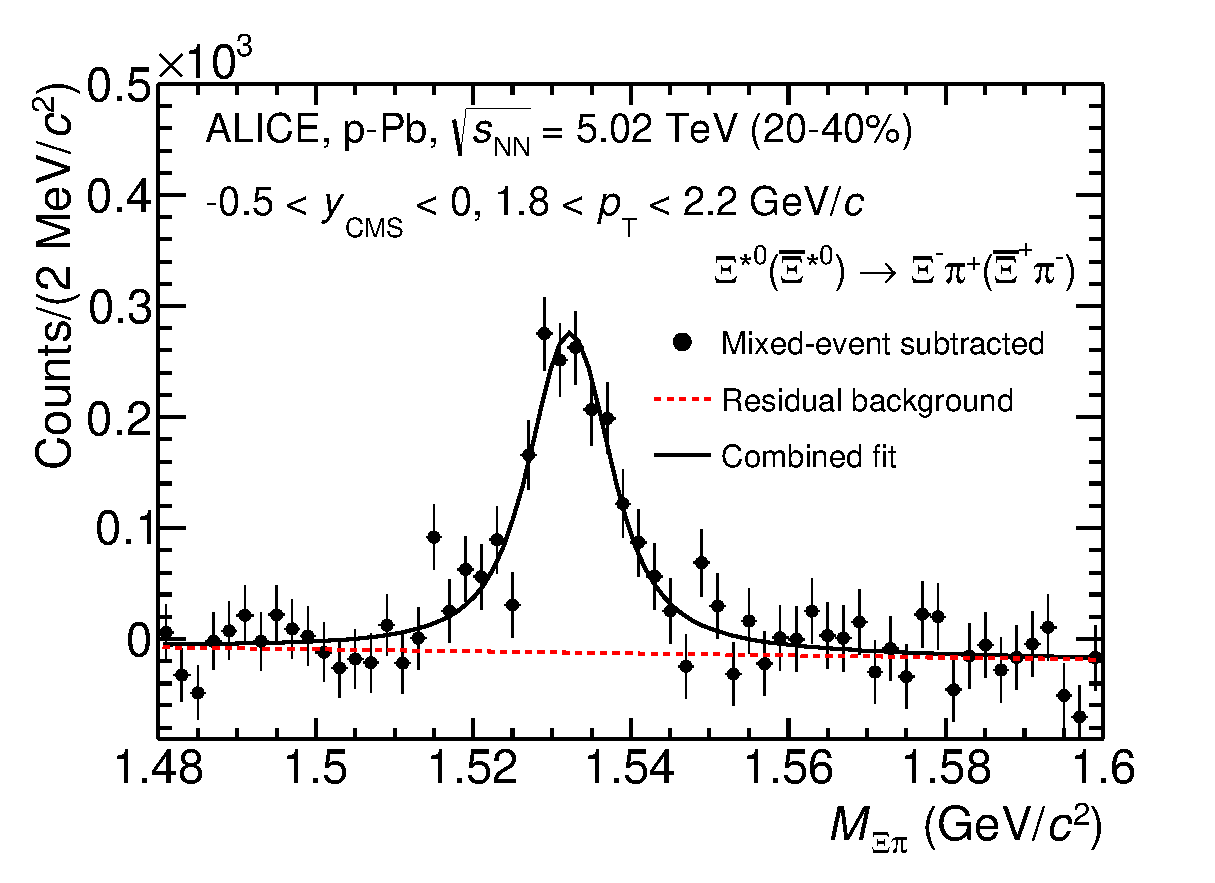
\includegraphics[width=12.0cm]{./Version1/FigChapter5/Extraction/SigpPb_After.eps}
\hspace{0.5cm}
\label{fig:sigpPba} 
\caption{ The invariant mass distribution after subtraction of the mixed-event background in p--Pb collisions. 
The solid curve represents the combined fit, while the dashed line describes the residual background.}
\end{center}
\end{figure}


\begin{figure}[htbp]
\begin{center}
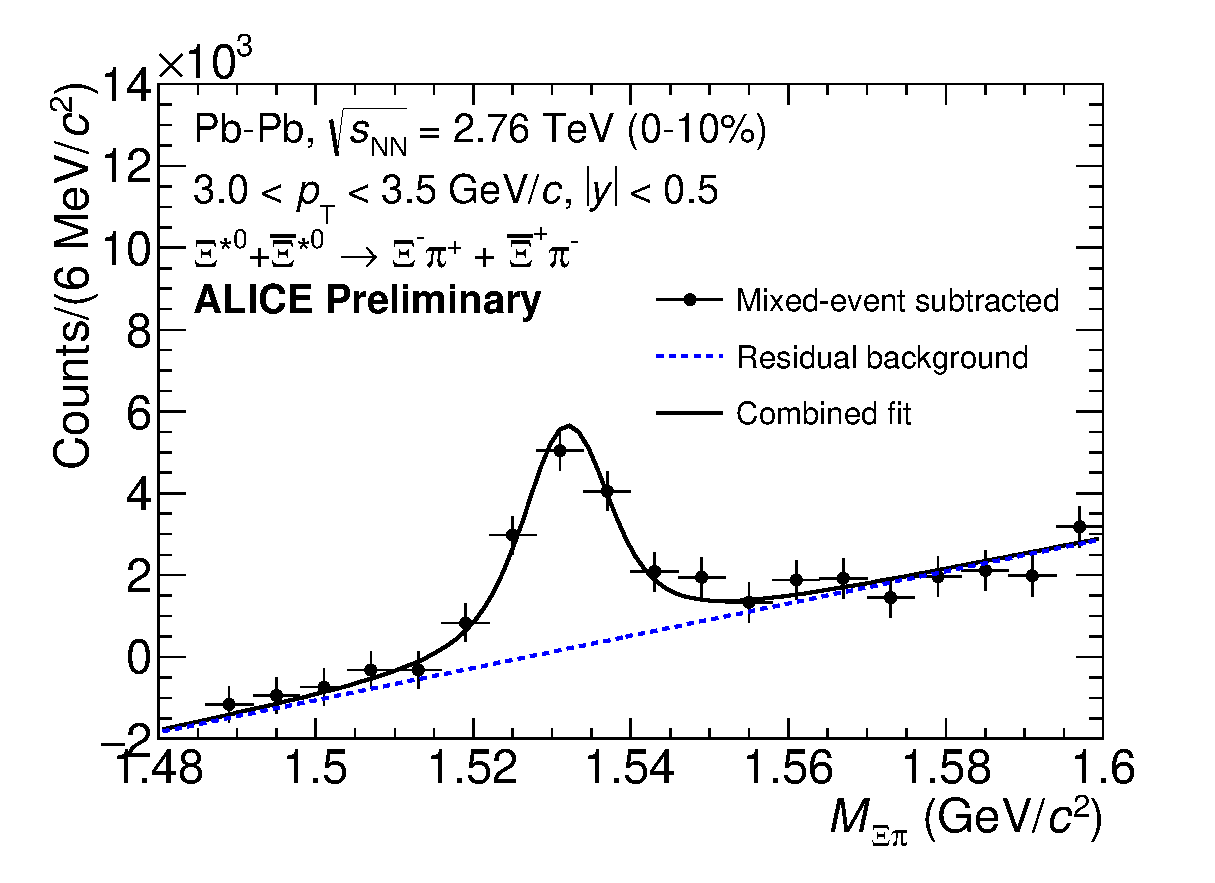
\includegraphics[width=12.0cm]{./Version1/FigChapter5/Extraction/SigPbPb_After.eps}
\hspace{0.5cm}
\label{fig:sigpPba} 
\caption{ The invariant mass distribution after subtraction of the mixed-event background in Pb--Pb collisions. 
The solid curve represents the combined fit, while the dashed line describes the residual background.}
\end{center}
\end{figure}

The mass parameter of the Voigtian fit ($M_{0}$) is left free within the fit range (1.48 \Gmass and 1.59 \Gmass). The overall invariant mass width of the Voigtian function is governed by 2 parameters: $\sigma$ and $\Gamma_{0}$. The $\sigma$ describes the broadening of the peak due to finite detector resolution while $\Gamma$ describes the intrinsic width of the resonance itself. The $\Gamma_{0}$ is fixed to the PDG value of 9.1 \mmom for the\xis. Because of lack of statistics, the $\sigma$ can be over estimated. Therefore the $\sigma$ parameter is fixed to value derived from $\sigma$ in MB events which has largest statistics. The $\sigma$ as function of \pt distribution in MB events is shown in Figure. \ref{fig:sigma} and we also report invariant mass of \xis as function of \pt in Figure. \ref{fig:mass}. The \xis raw yields have been extracted from the fit for the 4 multiplicity bins (+ NSD events) in p--Pb and 4 centrality bins in Pb--Pb collisions and the yields as function of \pt are shown in Figure \ref{fig:rawyield}.



\begin{figure}[htbp]
\begin{center}
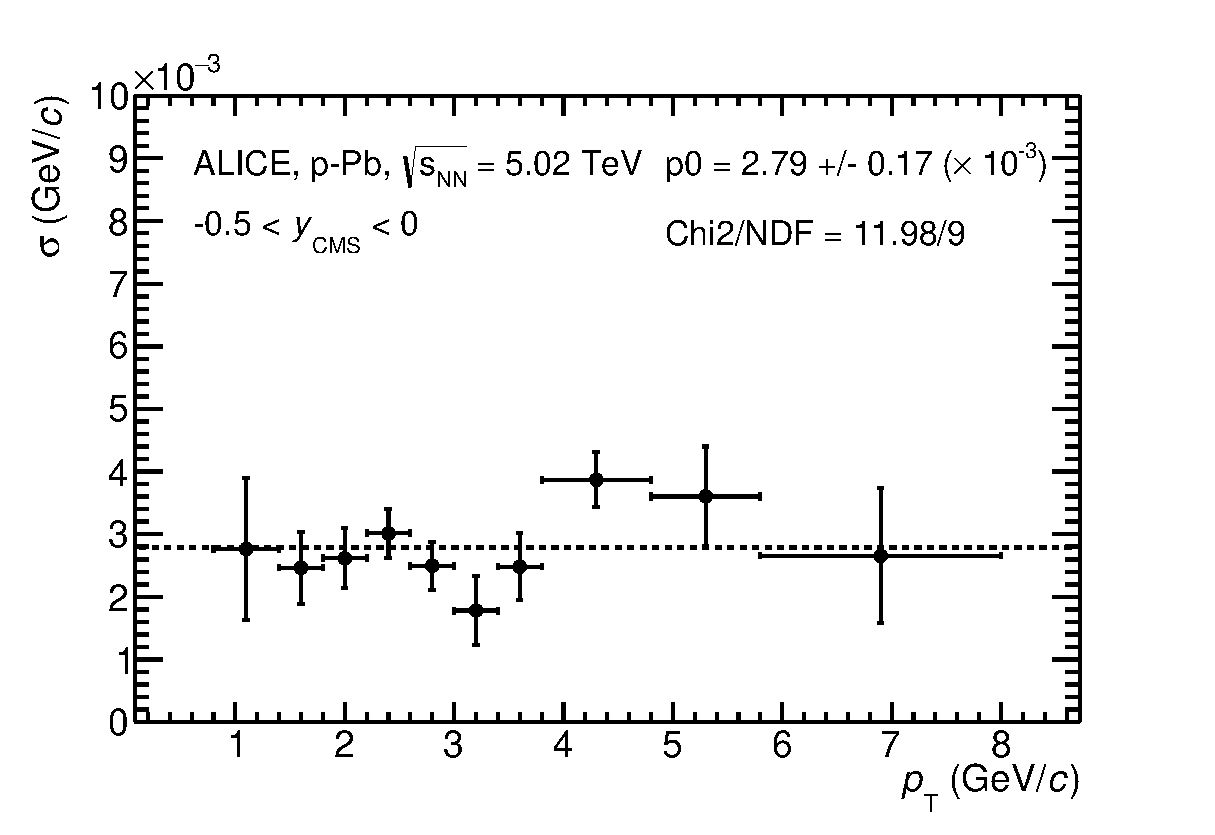
\includegraphics[width=10.0cm]{./Version1/FigChapter5/Extraction/pPbWidthMB.eps}
\hspace{0.5cm}
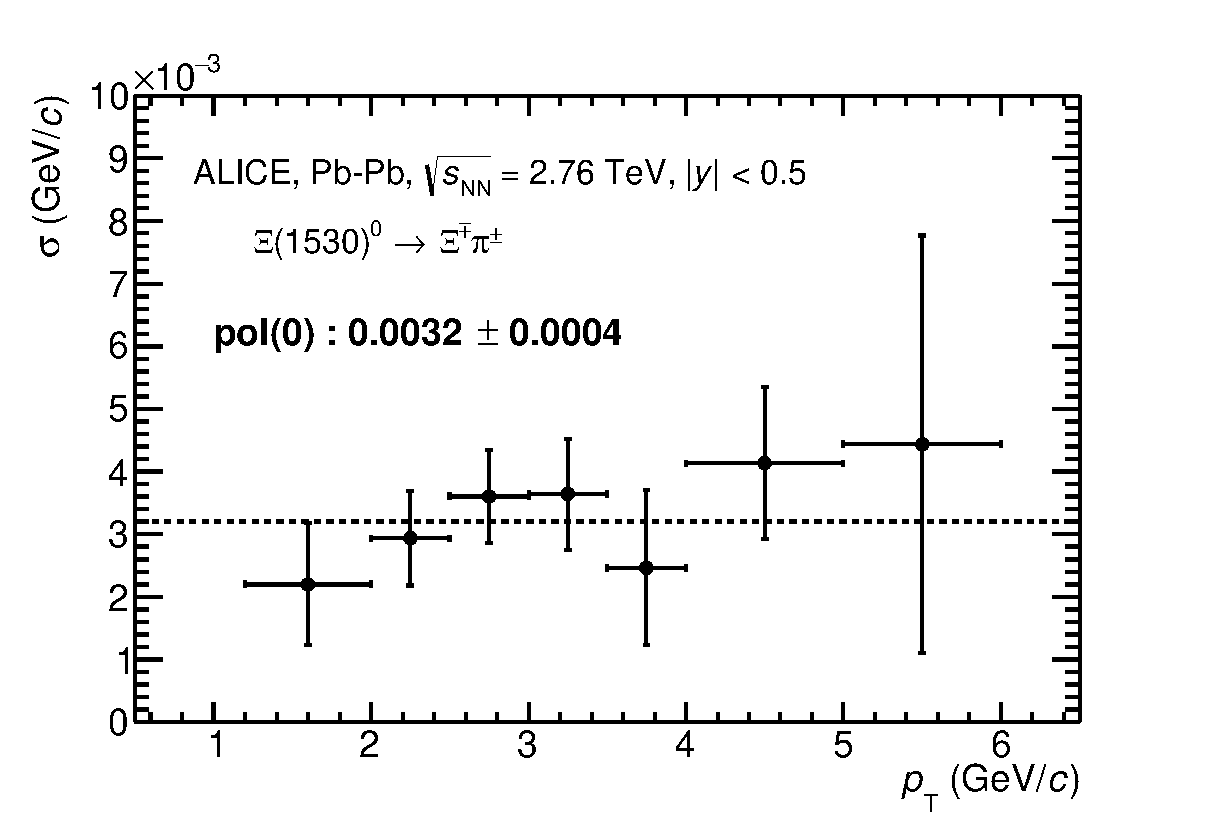
\includegraphics[width=10.0cm]{./Version1/FigChapter5/Extraction/PbPbWidthMB.eps}
\caption{$\sigma$ fit parameters as a function of \pt in MB in p--Pb collisions (top) and in Pb--Pb collisions (bottom).} 
 \label{fig:sigma}
\end{center}
\end{figure}



\begin{figure}[htbp]
\begin{center}
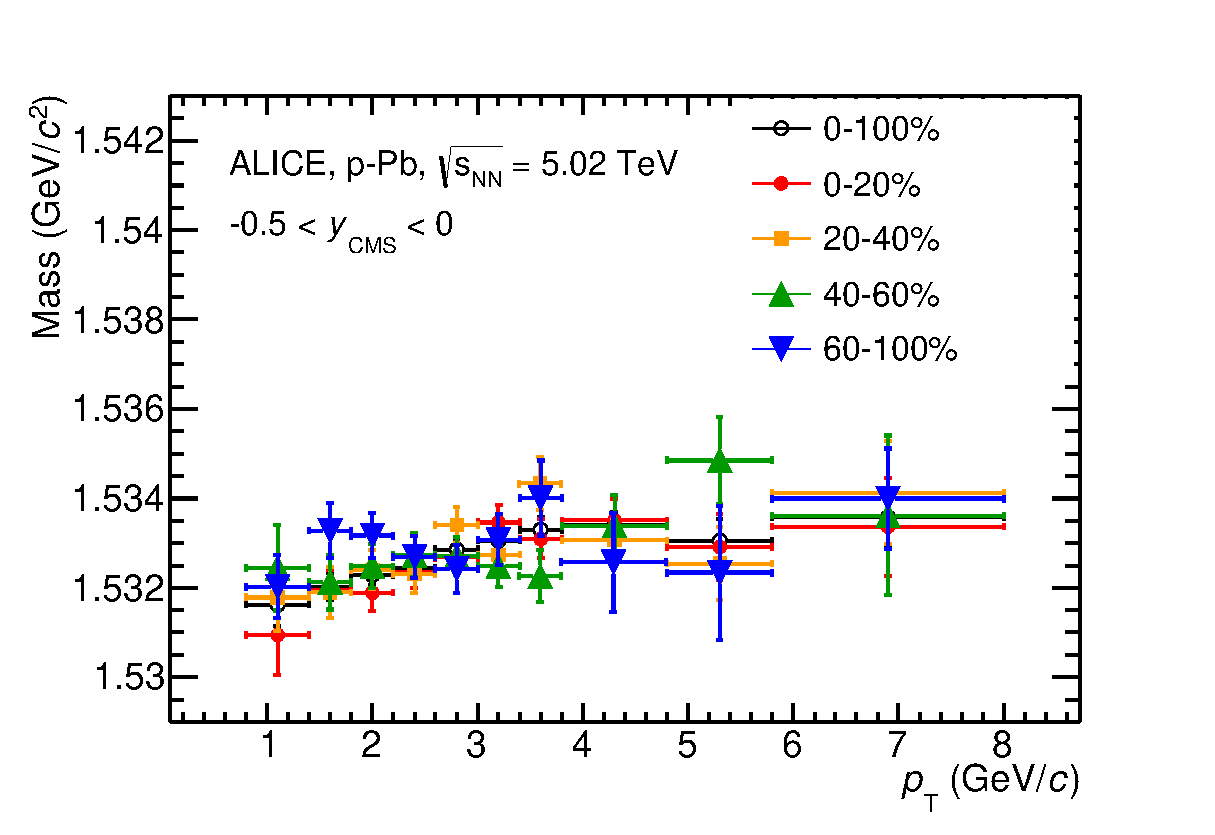
\includegraphics[width=10.0cm]{./Version1/FigChapter5/Extraction/pPbMass.eps}
\hspace{0.5cm}
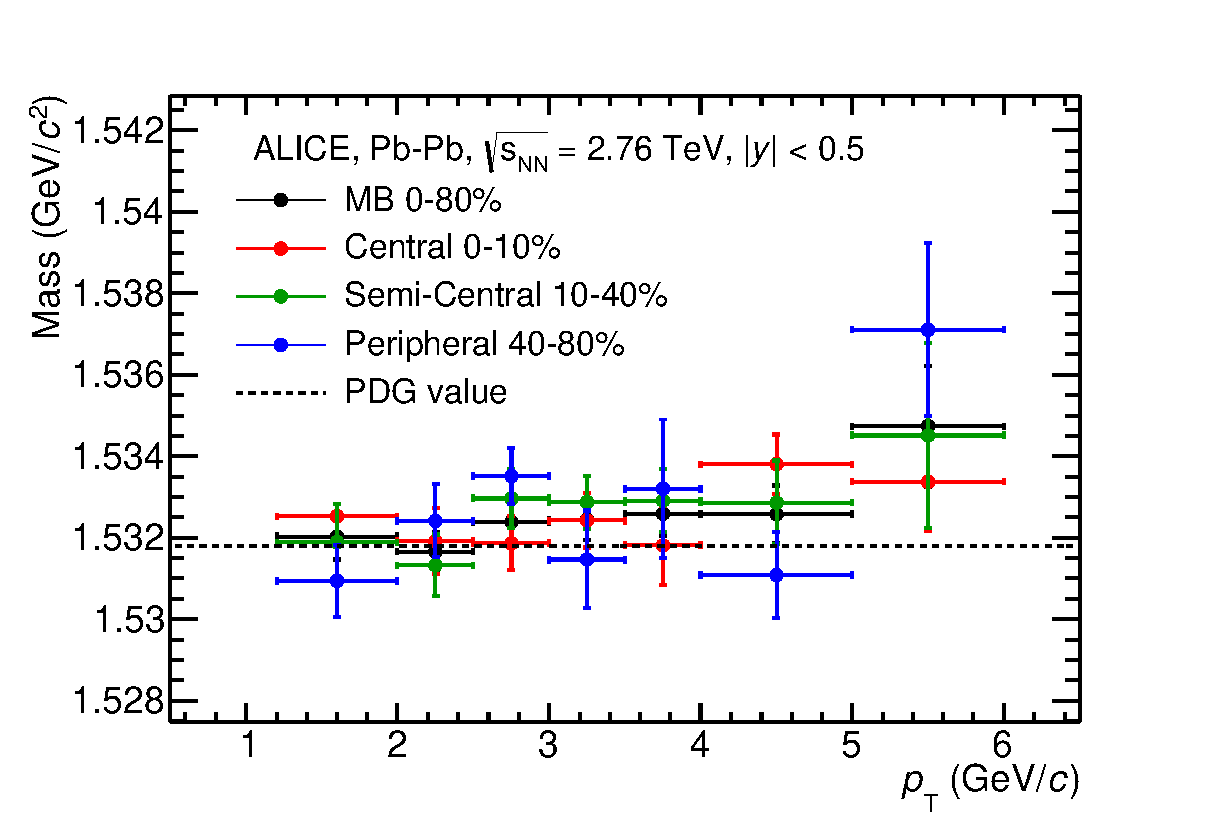
\includegraphics[width=10.0cm]{./Version1/FigChapter5/Extraction/PbPbMass.eps}
\caption{\xis-mass obtained from fit of the Voigtian peak as a function of \pt in each multiplicity classes in p--Pb collisions (top) and the different centrality classes in Pb--Pb (bottom).} 
 \label{fig:mass}
\end{center}
\end{figure}


\begin{figure}[htbp]
\begin{center}
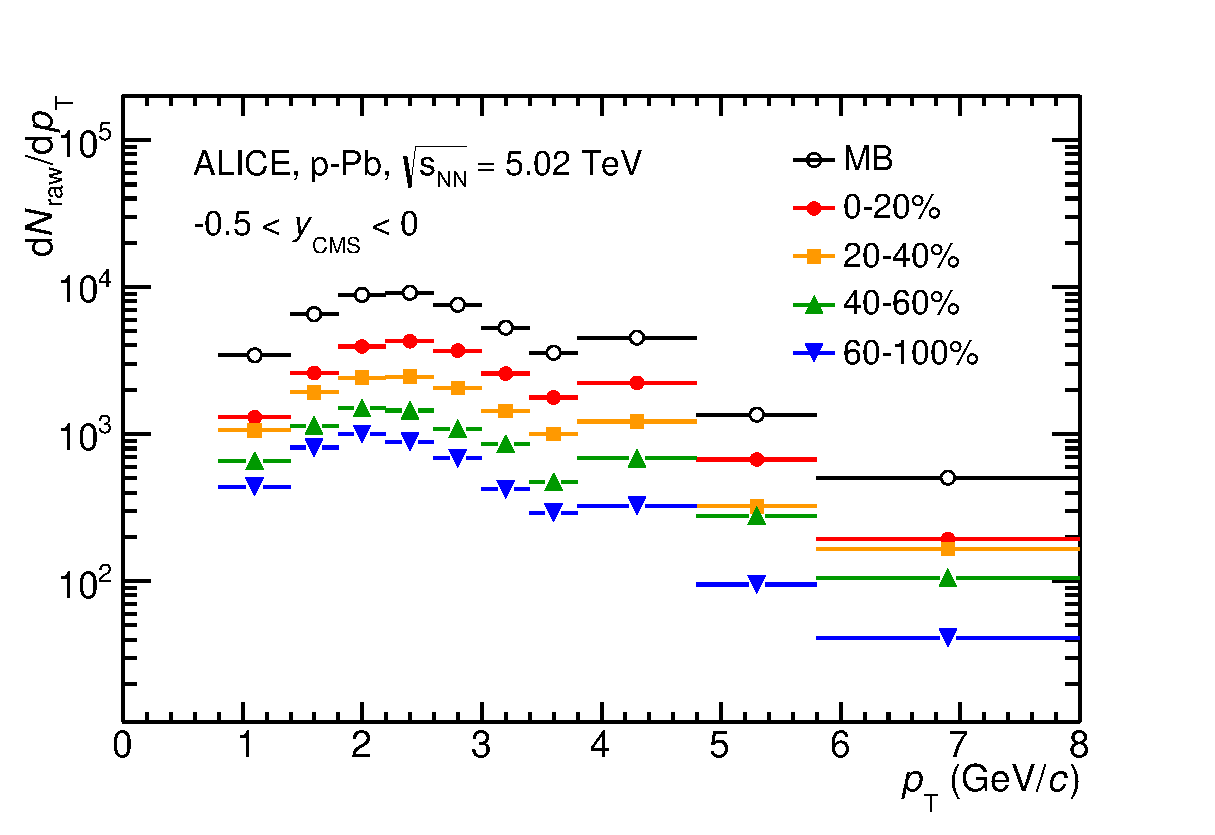
\includegraphics[width=10.0cm]{./Version1/FigChapter5/Extraction/pPbRawYield.eps}
\hspace{0.5cm}
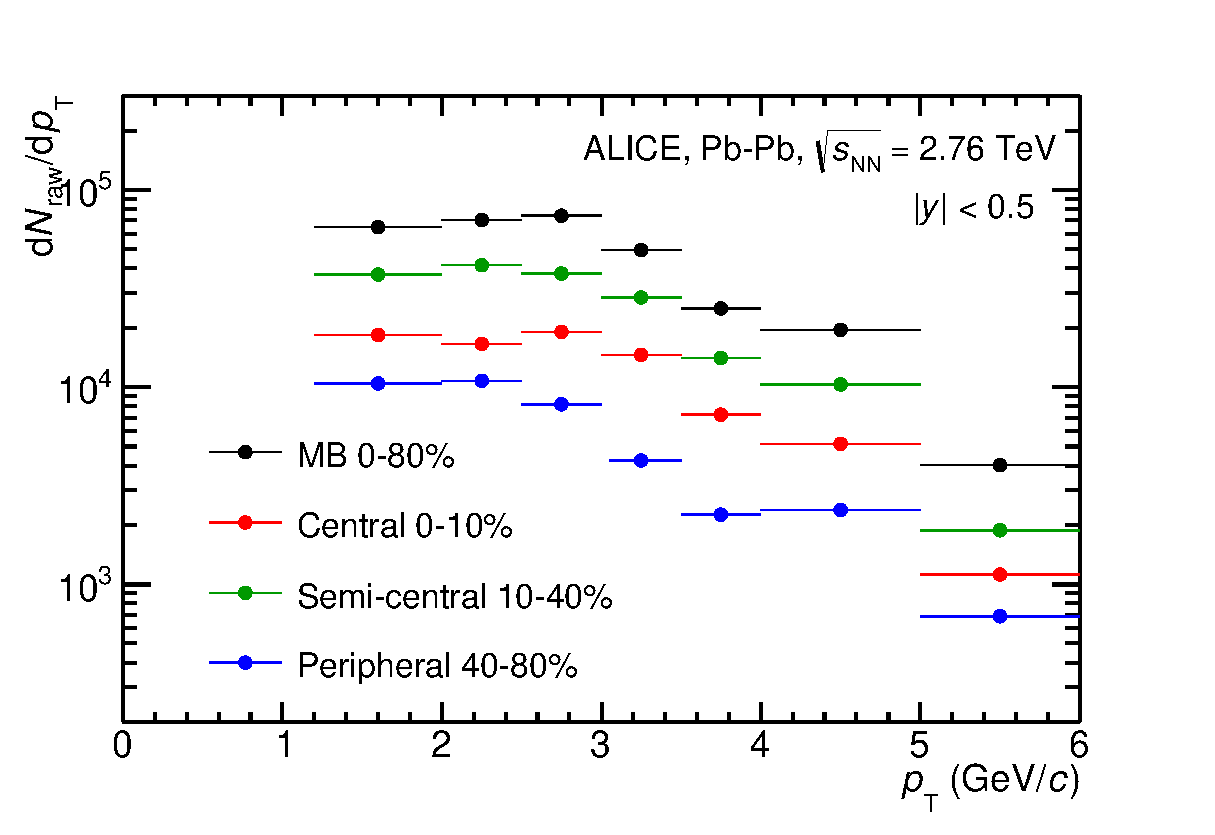
\includegraphics[width=10.0cm]{./Version1/FigChapter5/Extraction/PbPbRawYield.eps}
\caption{\xis-raw spectra obtained from fit of the Voigtian peak and a polynomial residual background for different multiplicities in p--Pb collisions (top) and Pb--Pb collisions (bottom). Only the statistical error is reported.} 
 \label{fig:rawyield}
\end{center}
\end{figure}





\newpage
\subsection{Efficiency correction}\label{sec:MC} 
The raw yields were corrected for the geometrical acceptance and the reconstruction efficiency
(A $\times$ $\epsilon$) of the detector (Figure.~\ref{fig:pPb:efficiency}). By using the DPMJET 3.05 event generator~\cite{cite:DPMJET} and the GEANT~3.21 package~\cite{cite:GEANT}, a sample of about 100 million p--Pb events was simulated and reconstructed in order to compute the corrections. The distributions of $A\times\epsilon$ were obtained from the ratio between the number of reconstructed $\Xi^{*0}$ and the number of generated particle in the same \pt~and rapidity interval. Since the correction factors for different multiplicity classes are in agreement with those from MB events within statistical uncertainty, the latter were used for all multiplicity classes.

\begin{figure}[htbp]
\begin{center}
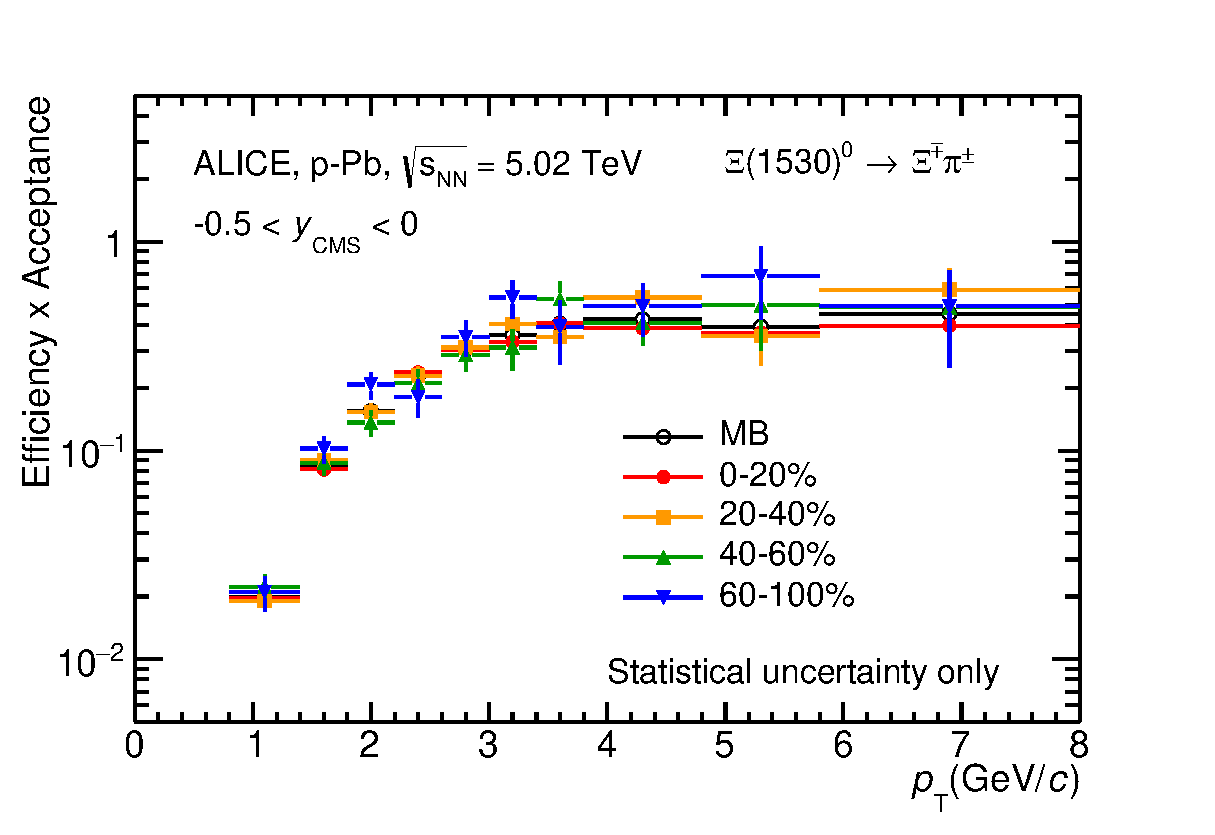
\includegraphics[width=10.0cm]{./Version1/FigChapter5/MC/Efficiency.eps}
\caption{\xis-raw spectra obtained from fit of the Voigtian peak and a polynomial residual background for different multiplicities. Only the statistical error is reported.} 
 \label{fig:pPb:efficiency}
\end{center}
\end{figure}


Because the generated $\Xi(1530)^{0}$ spectra have different shapes than the measured \xis spectra, it is necessary to weight the generated and reconstructed \xis spectra in these simulations. Fig. \ref{fig:pPb:datagenrec} shows the generated and reconstructed \xis spectra plotted with the (corrected) measured \xis spectrum for MB events and the Levy fit of that measured spectrum. The generated and measured \xis spectra have  different behaviours for the range 0.5 $<$ $p_{\mathrm{T}}$ $<$ 1 GeV/$c$. The generated \xis spectrum decreases with increasing \pt over this range, while the fit of the measured \xis spectrum reaches a local maximum in this range. The correction $\epsilon$ is observed to change rapidly over this \pt range. It is therefore necessary to weight the generated spectrum so that it has the shape of the measured  \xis  spectrum (and to apply corresponding weights to the reconstructed \xis spectrum). An iterative procedure is performed to determine the correct weighting (and therefore the correct $\epsilon$). 
\begin{figure}[htbp]
\begin{center}
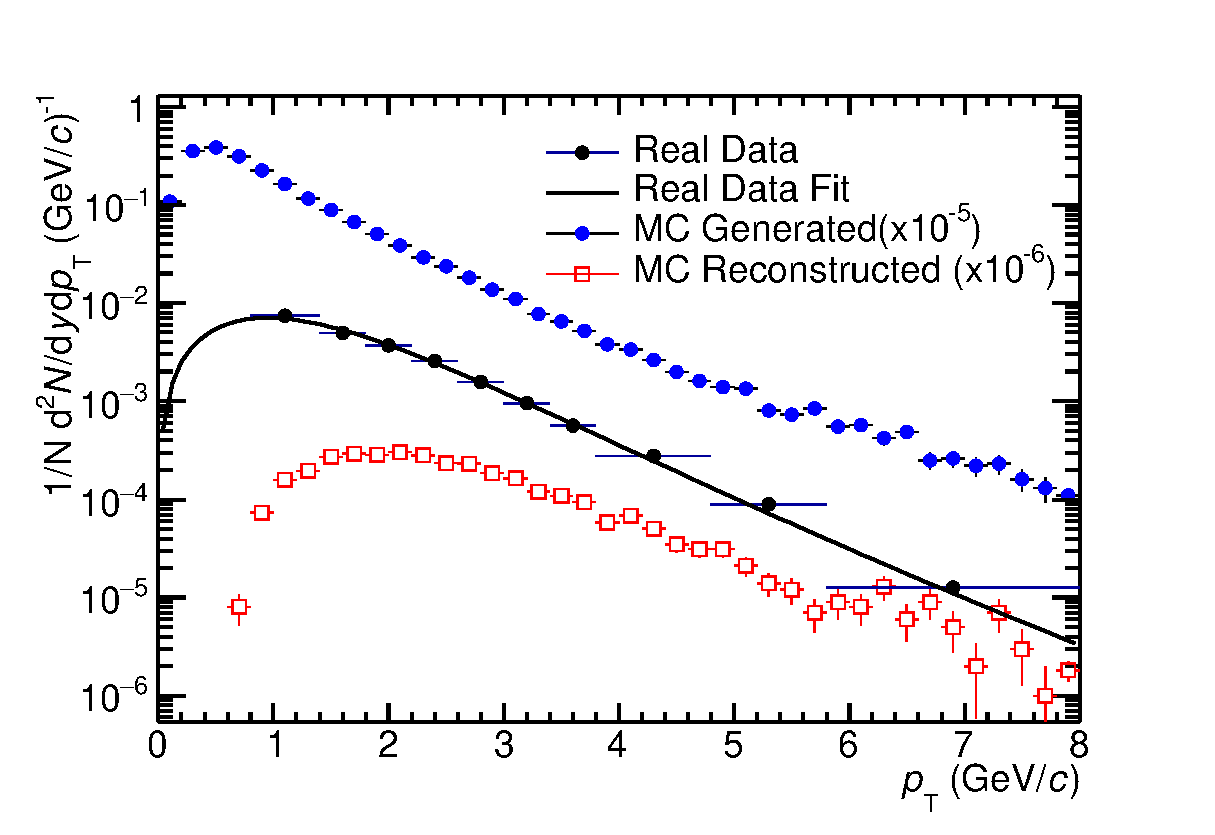
\includegraphics[width=10.0cm]{./Version1/FigChapter5/MC/Weighting.eps}
\caption{Real corrected \xis spectrum (black) for the minimum bias with Levy fit (black curve). Also shown are the unweighted generated (blue) and reconstructed (red) \xis spectra.}
\label{fig:pPb:datagenrec}
\end{center}
\end{figure}

\begin{enumerate}
\item The unweighted $\epsilon$ is calculated.
\item This $\epsilon$ is used to correct the measured xis spectrum.
\item The corrected \xis spectrum is fit.
\item This fit is used to weight the simulated xis spectra. A \pt dependent weight is applied to the generated xis spectrum so that it follows the fit. The same weight is applied to the reconstructedxis spectrum.
\item The (weighted) $\epsilon$ is calculated.
\item Steps 2-5 are repeated (with the weighted $\epsilon$ from step 5 used as the input for step 2) until the $\epsilon$ values are observed to change by $<$ 0.1\% (relative) between iterations. It is observed that four iterations are sufficient for this procedure to converge.
\end{enumerate}

Finally, the re-weighted efficiency is obtained and the distribution as function of \pt is shown in Figure \ref{fig:pPp:mbefficiency}.

\begin{figure}[htbp]
\begin{center}
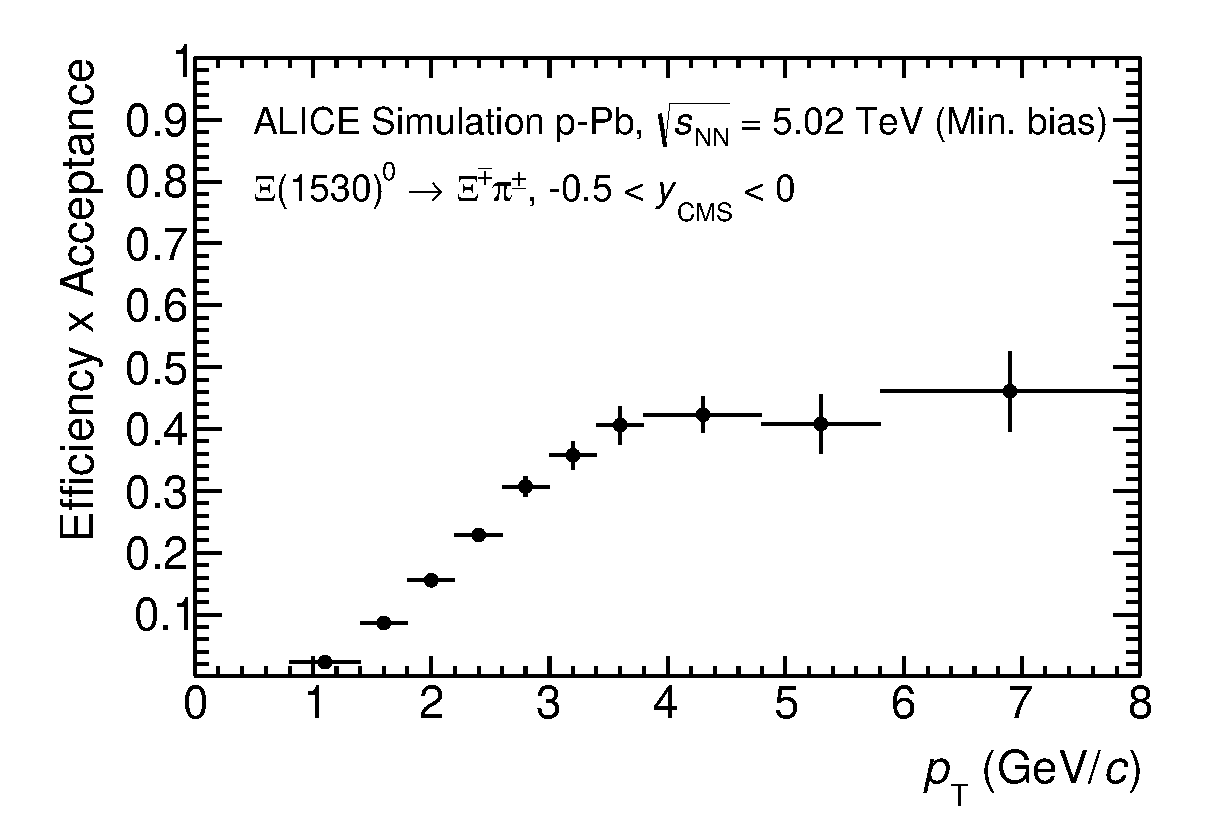
\includegraphics[width=10.0cm]{./Version1/FigChapter5/MC/MBEfficiency.eps}
\caption{Efficiency as a function of \pt in minimum bias events in p--Pb collisions.} 
 \label{fig:pPp:mbefficiency}
\end{center}
\end{figure}


In order to obtain the correction factor dedicated in Pb--Pb collisions, MC events are generated using Heavy Ion Jet Interaction Generator (HIJING). The generated events are passed through a GEANT3 model of the ALICE experiment with a realistic description of the detector response. Because we have observed centrality dependent efficiency, the centrality dependent efficiencies have been applied to get corrected raw yield. The reweighing approach which was used to correct the efficiency in p--Pb is also applied to the efficiency obtained in Pb-Pb. 

\begin{figure}[htbp]
\begin{center}
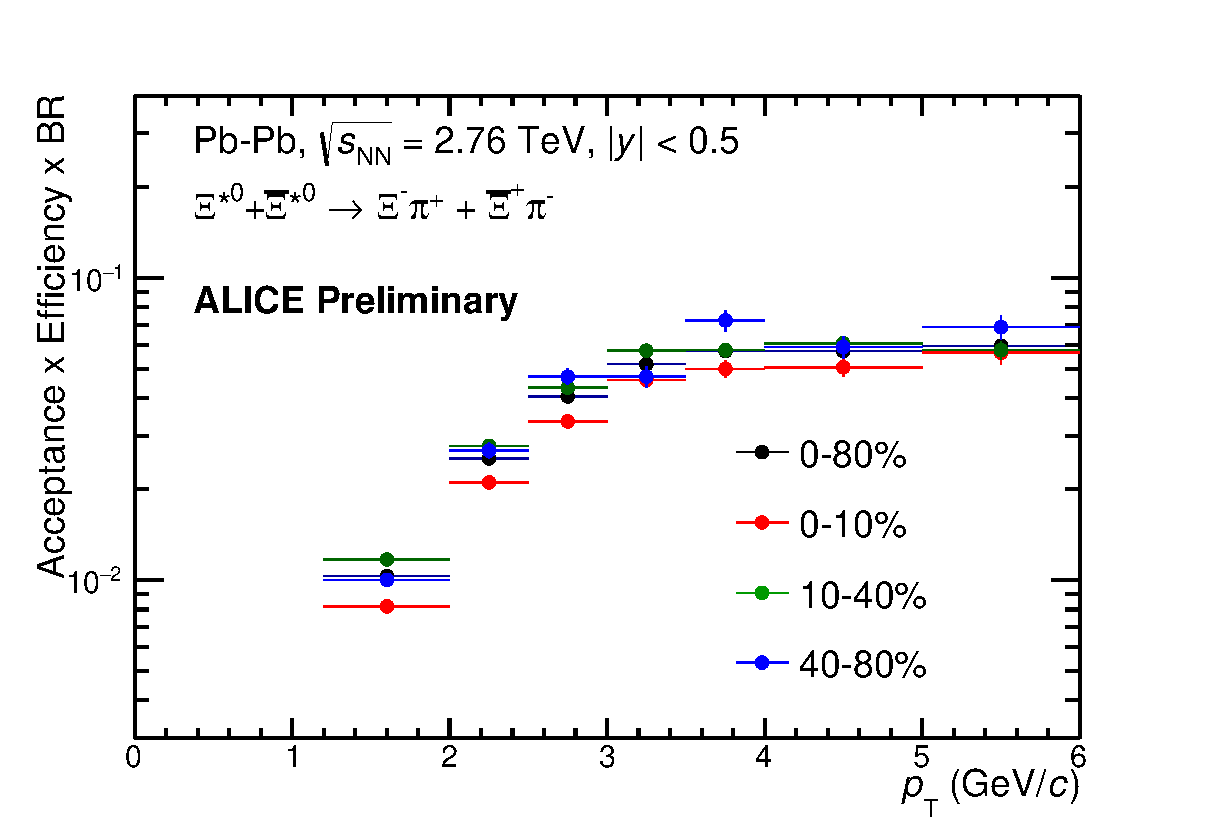
\includegraphics[width=10.0cm]{./Version1/FigChapter5/MC/PbPbEfficiency.eps}
\caption{Efficiency as a function of \pt in different centrality classes in Pb--Pb collisions} 
 \label{fig:PbPb:efficiency}
\end{center}
\end{figure}


\newpage
\subsection{Corrected \pt-spectra}\label{sec:pPb:spectra} 

The $p_{\mathrm{T}}$ spectrum is by the number of produced particles of a given type in the desired interval of phase-space divided by the number of inelastic collisions. The spectrum is calculated as:

\begin{equation}
\frac{1}{N} \times \frac{d^{2}N}{dydp_{T}} = \frac{1}{N_{E,PhysSel}} \times \frac{N_{raw}}{dp_{T}dy}  \frac{1}{\epsilon} \frac{N_{total}^{MC}}{N_{post-PV cut}^{MC}}   ,
\end{equation}

where N$_{E}$ represent the number inelastic collisions, the $\frac{dN}{dydp_{T}}$ is the yield  per range of rapidity $y$, per range in \pt. On the right hand side N$_{E,PhysSel}$ is the number of events counted by the physics selection trigger. N$_{raw}$ is the raw extracted number of particle in the rapidity and \pt bin of width $\Delta y$ = 0.5 in p--Pb ($\Delta y$ = 1.0 in Pb--Pb) and $\Delta$p$_{T}$, respectively. $\epsilon$ is the reconstruction efficiency estimated from Monte Carlo simulations. $\frac{N_{total}^{MC}}{N_{post-PV cut}^{MC}}$ is the ratio of the total number of particle from MC divided by the number of particle from MC after the Primary-Vertex cut is imposed. It takes into account the fraction of particle lost after imposing the PV cut. We notice that for minimum-bias results in p--Pb, we adopted a normalisation such that to provide result from non-single diffractive(NSD) cross-section. The normalisation factor is 0.964 \cite{cite:KphipPb}. The obtained spectrum at MB and the spectrums from different multiplicity classes in p--Pb are shown in Figure \ref{fig:pPb:rawspectra} and different centrality classes in Pb--Pb are shown in Figure \ref{fig:PbPb:rawspectra}.

\begin{figure}[htbp]
\begin{center}
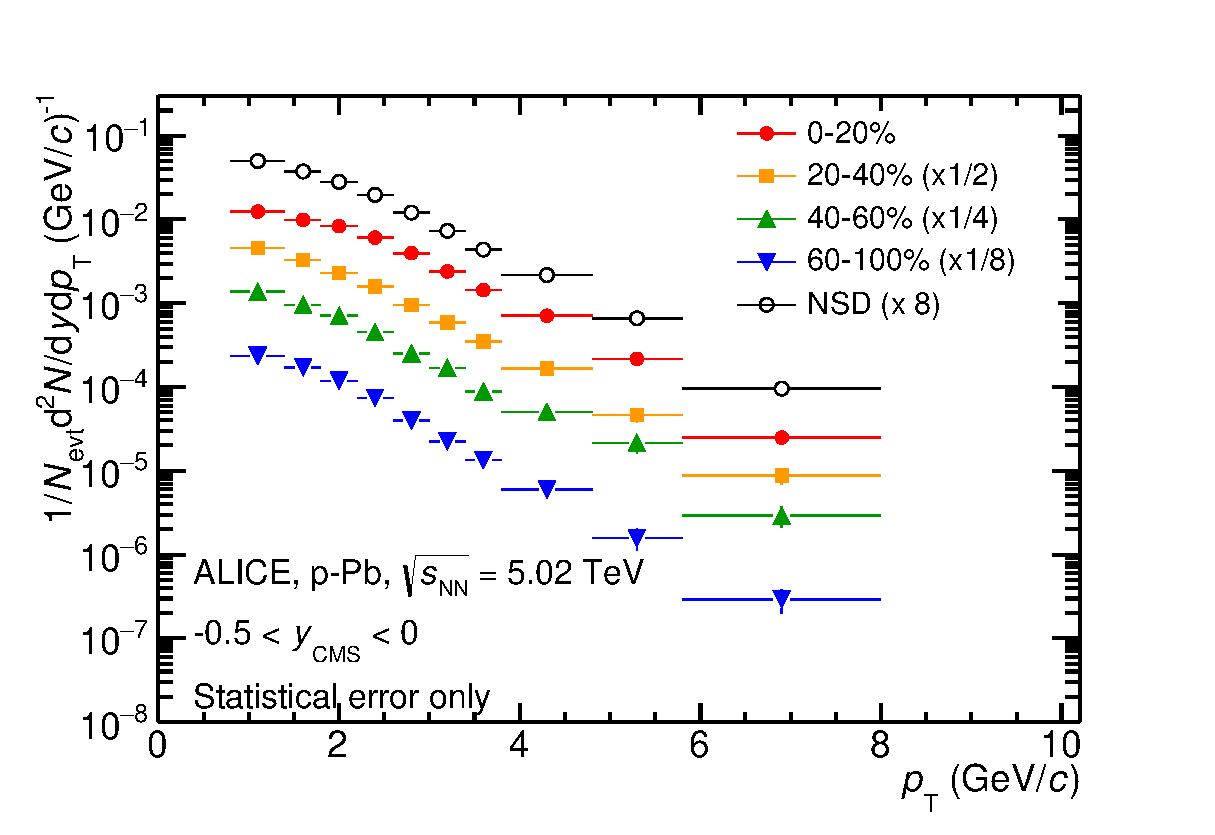
\includegraphics[width=10.0cm]{./Version1/FigChapter5/Spectra/StatSpectrapPb.eps}
\caption{Corrected \pt-spectra of \xis in NSD and different multiplicity classes in p--Pb collisions.} 
 \label{fig:pPb:rawspectra}
\end{center}
\end{figure}

\begin{figure}[htbp]
\begin{center}
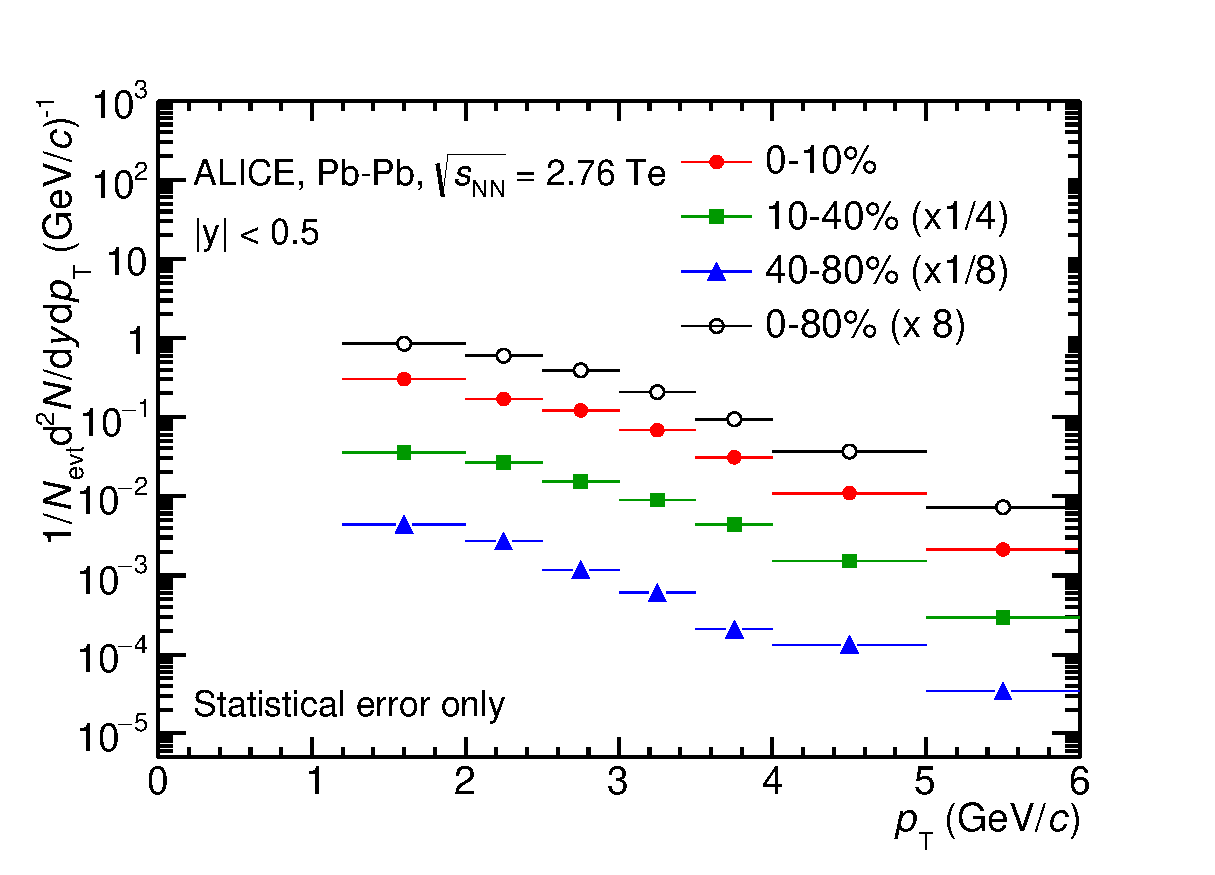
\includegraphics[width=10.0cm]{./Version1/FigChapter5/Spectra/StatSpectraPbPb.eps}
\caption{Corrected \pt-spectra of \xis in different centrality classes in Pb-Pb collisions.} 
 \label{fig:PbPb:rawspectra}
\end{center}
\end{figure}



\newpage
\subsection{Systematic uncertainties}\label{sec:sys} 


The systematic uncertainties are calculated in seven principle groups. The procedure to obtain the systematic uncertainties is performed many times by varying the possible permutation of the analysis parameter.The general strategy for evaluating systematic uncertainties is described as following:

\begin{enumerate}
\item Choose one set of parameters for the analysis as default
\item Observe the deviation of yield when one parameter is changed
\item The systematic uncertainty is calculated for a given source as the RMS deviation of the available sources.
\item The total systematic uncertainty, taking into account all the different sources, is the sum in quadrature of each source.
\end{enumerate}

To study the systematic effect we repeat the measurement by varying one parameter at a time. 
A Barlow \cite{cite:Barlow} check has been performed for each measurement to verify whether it is due to a systematic effect or a statistical fluctuation. Let each measurement be indicated by ($\it{y}_{i}$$\pm$$\sigma_{i}$) and the central value (default measurement) by ($\it{y}_{c}$$\pm$$\sigma_{c}$), one can define $\Delta\sigma_{i}$ (Eq. \ref{eq:barlow}).


\begin{equation}
 \Delta\sigma_{i} = \sqrt(|\sigma_{i}^{2} - \sigma_{c}^{2}|)
 \label {eq:barlow}
\end{equation}

Then we calculate $\it{n}_{i}$ = $\Delta\it{y}_{i}$/ $\Delta\sigma_{i}$, where  $\Delta\it{y}_{i}$ = $|$$\it{y}_{c}$ - $\it{y}_{i}$$|$.
If $\it{n}_{i}$ $\leq$ 1.0 then the effects are due to the statistical fluctuation and if $\it{n}_{i}$ $>$ 1.0 we apply consistency check. Since the alternate and default measurements are not statistically independent, an alternate measurement which is statistically consistent with the default measurement should not be used in calculating a systematic uncertainty. The difference between the two measurements is $\Delta$ = $\it{y}$$_{c}$ - $\it{y}$$_{i}$. The difference in quadrature of the uncertainties is calculated by Eq. \ref{eq:barlow}. 
It could be possible to check if $\Delta$$<$ $\sigma$ and exclude such cases from the systematic uncertainties. However, there can be statistical fluctuations for which $\Delta$$>$ $\sigma$. If the variations between the default and alternate measurements are purely statistical, the distribution of $\Delta$$/$$\sigma$ should be a Gaussian with a mean value that is consistent with zero and a deviation $\sigma$ consistent with unity. In this analysis, if the mean value is less than 0.1 and $\sigma$ is less than 1, the variation passes the consistency check.

Only the measurements which passed the Barlow check ($\it{n}_{i}$ $>$ 1) are used to determine the systematic uncertainty. For measurements N $>$ 2, the systematic uncertainty has been determined as the RMS (eqn. \ref{eq:rms}) of the available measurements. If N=2, the absolute difference is assigned as systematic uncertainty.

\begin{equation}
\delta y_{syst.}=\sqrt{\frac{1}{N}\sum_{i}(y_{i}-\overline{y})^{2}}
\label{eq:rms}
\end{equation}

Here N is the total number of available measurements including $\it{y}_{c}$ and $\overline{\it{y}}$ is the average of value of the measurements. The measurement did not pass Barlow check, zero systematic uncertainty has been assigned to the value.

By suing the way as explained above, all the main contributions to the systematic uncertainty of particle spectra have been studied. In particular those that comes from signal extraction, topological and kinematical selection cuts, track quality selection and n$\sigma$ TPC PID variation. the meaning of each source of systematic uncertainty studied is described in the following: \\

\textbf{Signal extraction}\\
We have extracted the signal with varying the yield calculating method which contains the method of signal extraction by integrating the Voigtian fit function and bin counting. We also have varied the normalisation range which is related to the invariant mass region where the mixed events distribution is scaled to subtract the combinatorial background and different background estimator such as Like-Sign distribution and polynomial fit was taken account into the systematic source of signal extraction. The systematic uncertainty from signal extraction is sum in quadrature of three sources. \\


\textbf{Topological selection}\\
To evaluate the stability of the chosen set of values for the topological cuts, loose and tight cuts have beed defined in order to vary by $\pm$10\% respectively. The parameters are changed once at a time. Total systematic uncertainty from topological selection is calculated by summation in quadrature of nine sources.\\


\textbf{TPC N$_{cluster}$ selection}\\
The selection performed for the daughter tracks of the cascade is that N$_{cluster}$ is larger than 70 and the value has been varied to 60 and 80 in order to estimate the systematic uncertainty  due to this selection. \\


\textbf{TPC $\mathrm{d}E/\mathrm{d}x$ selection}\\
In order to evaluate any potential effect due to the TPC $\mathrm{d}E/\mathrm{d}x$ selection (U$_{PID}$), the N$_{\sigma}$ selection was varied with N = 2.5 and 3.5. \\


\textbf{\pt~shape correction}\\
As described in Section \ref{sec:MC}, due to the different shape of the measured and generated \xis spectra, we have applied reweighing procedure to the generated spectra to have same shape and this correction is added into contributor of systematic uncertainty as \pt~shape correction.\\

\textbf{Mass window range selection}\\
In order to select $\Xi^{\pm}$ which is daughter particle of \xis, we apply the mass window $\pm$7 \mmass~around \xis mass on $\Lambda$$\pi$ invariant mass distribution. The boundaries has been varied to $\pm$6 \mmass~and $\pm$8 \mmass~to estimate systematic uncertainty.\\
 

\textbf{Vertex range selection}\\
The distribution of vertex-z is shown in Fig.\ref{fig:VzDistribution}. The cut on $|$Vz$|$ was varied from the nominal $\pm$10cm to $\pm$9cm, $\pm$11cm.\\

\textbf{Material Budget and hadronic cross section}\\
A possible source of uncertainty comes from the description of the material, active (detecting area) or dead (structure and cable), that the particles cross during their travel in the MC with respect to the real material present in the detector. Such description could affect the reconstruction efficiency in different aspects (e.g. multiple scattering, energy loss). The value estimated by $\Xi$ analysis \cite{cite:strangePbPb} has been used in this study which gives 4\% systematic uncertainty. In case of systematic uncertainty from hadronic cross section, we have inherited the value studied in previous measurement\cite{cite:trackingeffi} which amount is 1\%.\\

\textbf{Tracking efficiency}\\
Systematic uncertainties from tracking efficiency from ITS + TPC combined track were assigned as 3\% in p--Pb and  4\% in Pb--Pb collision system.\cite{cite:trackingeffi} \\
(https://twiki.cern.ch/twiki/bin/view/ALICE/TrackingEfficiencyCharged)\\


Finally, total systematic uncertainty is sum in quadrature of sources listed above. Figure \ref{fig:pPb:syserrortot} and Figure \ref{fig:pPb:syscent} show the total systematic uncertainty in minimum bias event and different multiplicity classes in p--Pb collisions, respectively. Again, Figure \ref{fig:PbPb:syserrortot} and Figure \ref{fig:PbPb:syscent} present the total systematic uncertainty in minimum bias event and different centrality classes in Pb--Pb collisions.


\begin{figure}[htbp]
\begin{center}
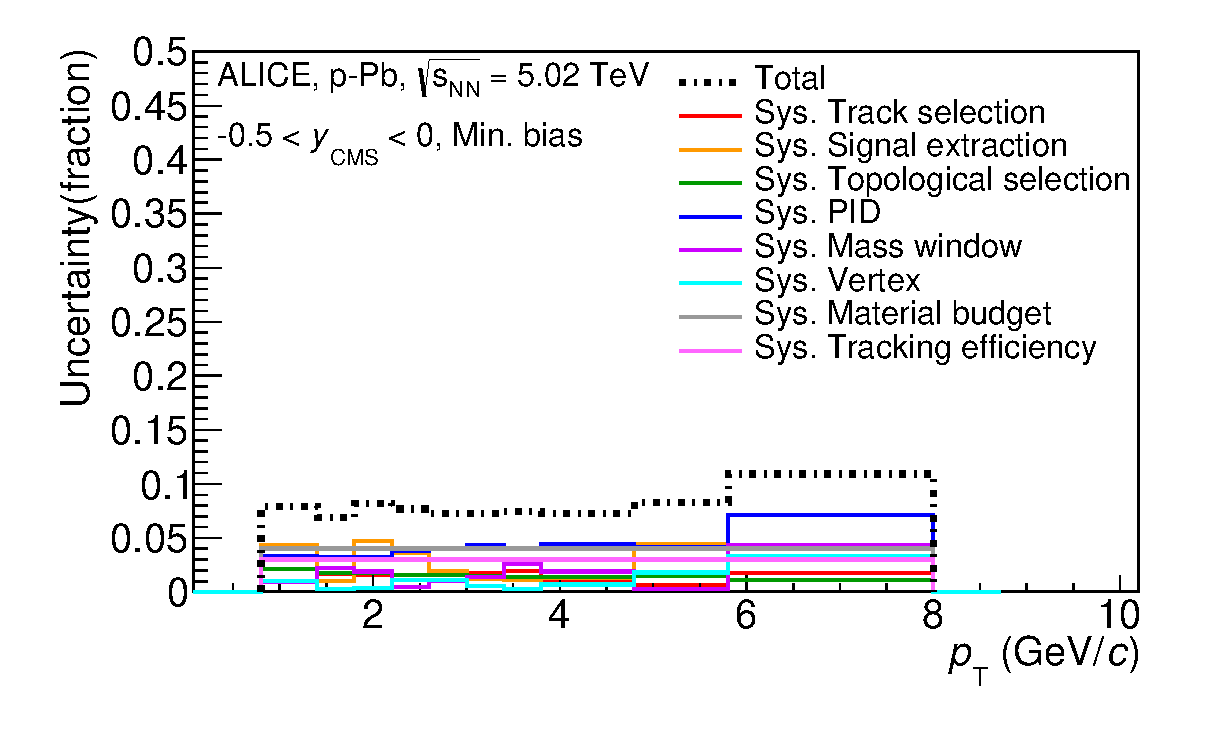
\includegraphics[width=12.0cm]{./Version1/FigChapter5/Systematic/pPbSysTotalFinal.eps}
\caption{Summary of the contributions to the systematic uncertainty in minimum bias events in p--Pb collisions. The dashed black line is the sum in quadrature of all the contributions.} 
\label{fig:pPb:syserrortot}
\end{center}
\end{figure}

\begin{figure}[htbp]
\begin{center}
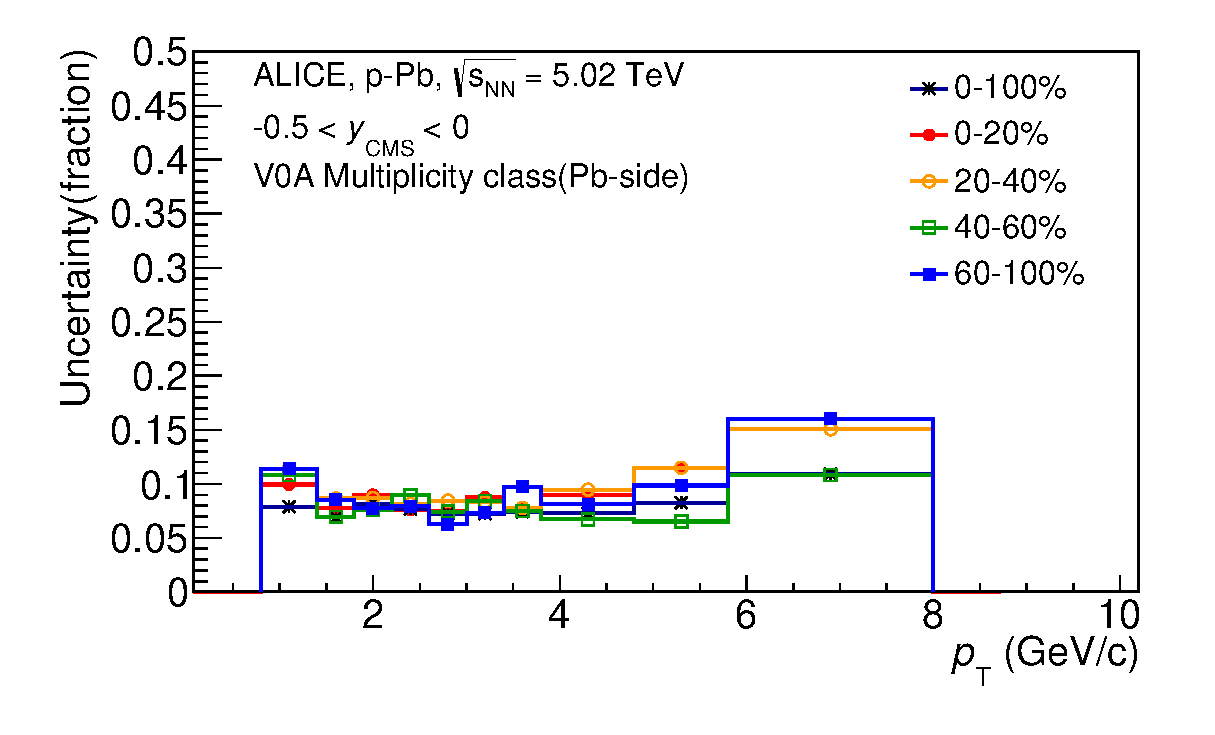
\includegraphics[width=12.0cm]{./Version1/FigChapter5/Systematic/pPbCent.eps}
\caption{Systematic uncertainties for each multiplicity classes in p--Pb collisions.} 
\label{fig:pPb:syscent}
\end{center}
\end{figure}


\begin{figure}[htbp]
\begin{center}
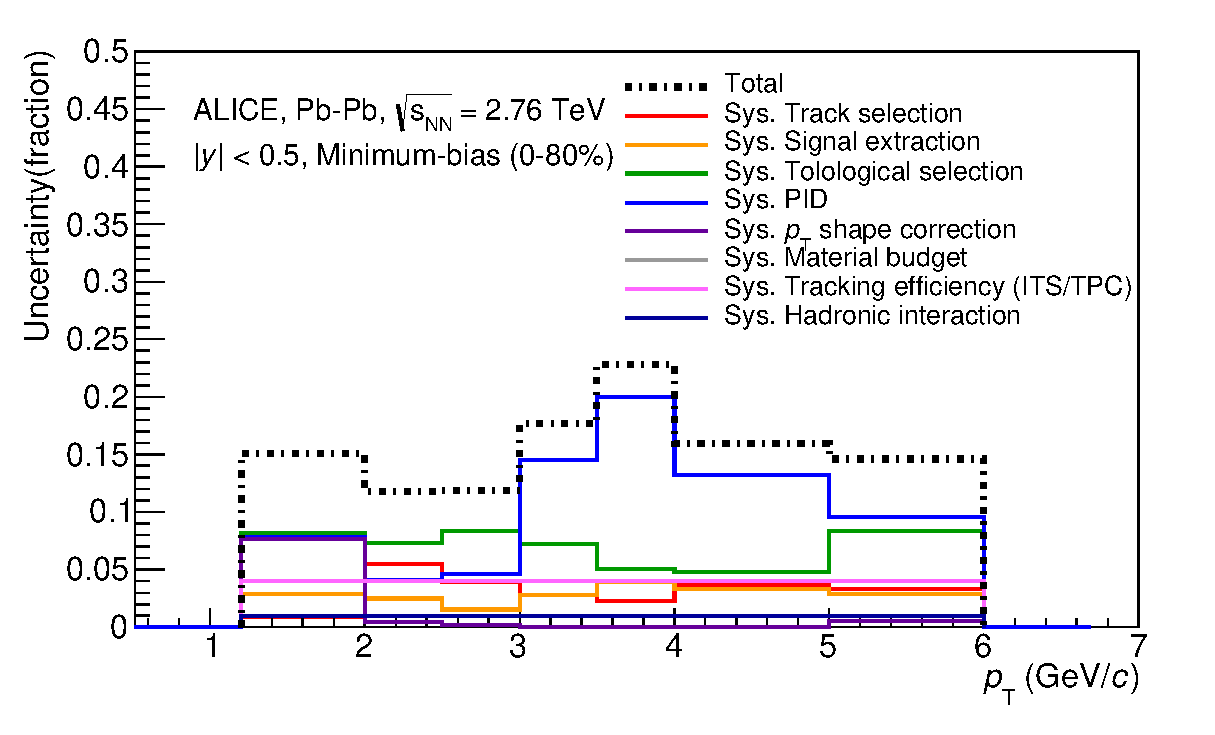
\includegraphics[width=12.0cm]{./Version1/FigChapter5/Systematic/PbPbSysTotalFinal.eps}
\caption{Summary of the contributions to the systematic uncertainty in minimum bias events in Pb--Pb collisions. The dashed black line is the sum in quadrature of all the contributions.} 
\label{fig:PbPb:syserrortot}
\end{center}
\end{figure}


\begin{figure}[htbp]
\begin{center}
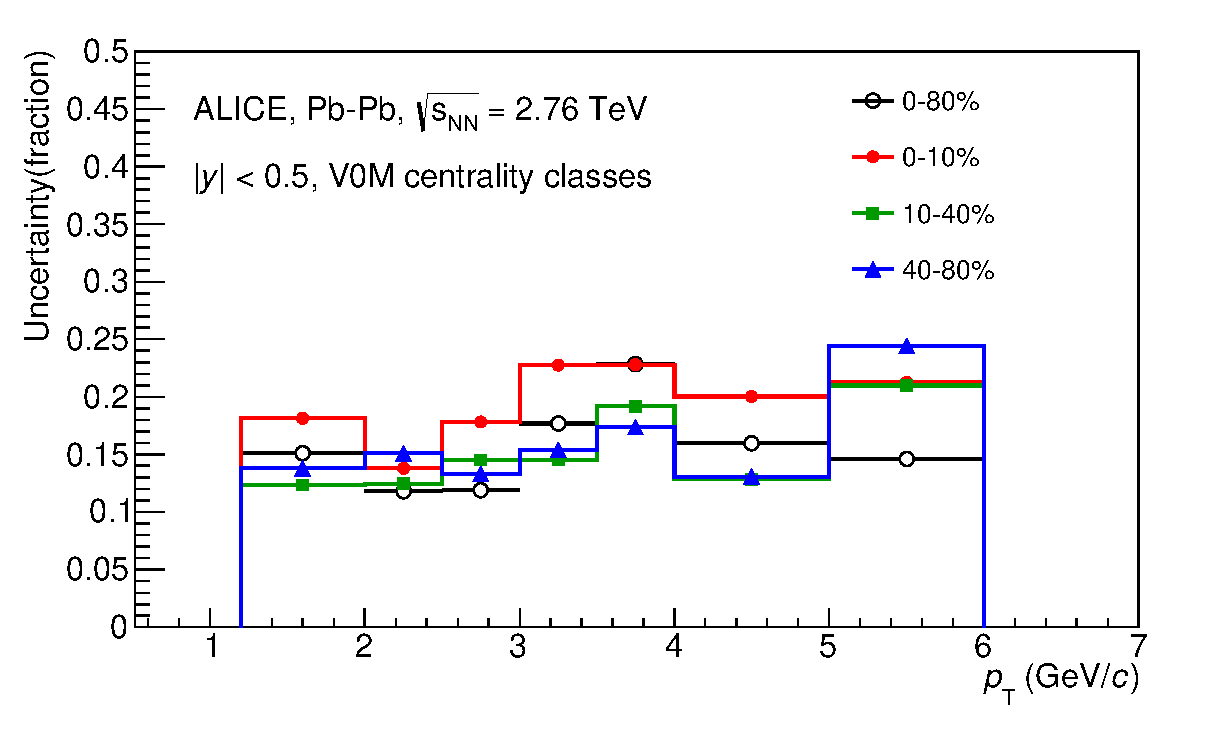
\includegraphics[width=12.0cm]{./Version1/FigChapter5/Systematic/PbPbCent.eps}
\caption{Systematic uncertainties for each multiplicity classes.} 
\label{fig:PbPb:syscent}
\end{center}
\end{figure}



\begin{table}[h!]
\centering
\begin{tabular}{lcc}
\hline\noalign{\smallskip}
Source of uncertainty &   p-Pb & Pb-Pb \\

\hline\noalign{\smallskip}
\pt-dependent & & \\
\hline\noalign{\smallskip}
Tracking efficiency & 3\% & 4\% \\
Tracks selection & 1-2\% &  1-5\% \\
Topological selection & 1-2\% & 5-8\% \\
PID  & 3-7\% &  4-20\% \\ 
Signal extraction & 1-5\% & 1-4\% \\
\pt~shape correction & - & 0-8\% \\
Mass window ($\Xi^\pm$)& 4\% &  - \\
Vertex selection & 3\% & - \\
\hline\noalign{\smallskip}
\pt-independent & & \\
\hline\noalign{\smallskip}
Hadronic interaction &  - &  1\% \\
Material budget  & 4\% &  4\% \\
Branching ratio  & 0.3\% & 0.3\% \\
\hline\noalign{\smallskip}
Total & 8-12\% & 9-25 \% \\
\hline\noalign{\smallskip}
\end{tabular}
\caption{Summary of the systematic uncertainties on the differential yield, \dndydpt. 
Minimum and maximum values in all \pt~intervals and multiplicity classes in p--Pb, centrality classes in Pb--Pb are shown for 
each source.}
\label{tab:sys}    
\end{table}


\newpage
\subsection{\xis~transverse momentum spectra}\label{sec:pPb:spectra} 
The raw yield shown in Figure \ref{fig:pPb:rawspectra} and \ref{fig:PbPb:rawspectra} have been corrected for efficiency as described in section \ref{sec:MC}. The measured spectra for (\xis+\xisb)/2 are reported in Figure \ref{fig:pPb:spectrasysstat} for p--Pb collisions and Figure \ref{fig:PbPb:spectrasysstat} for Pb--Pb collisions. The statistical and systematic uncertainties are reported respectively as the error bars and the boxes on the plot. The corrected yields for p--Pb collisions are measured with  0.8$<$ \pt $<$ 8.0 \gmom~while the yields for Pb--Pb collisions are obtained with 1.2 $<$ \pt $<$ 6.0 \gmom~due to difficulty of signal extraction in low and high \pt~region. 

\begin{figure}[htbp]
\begin{center}
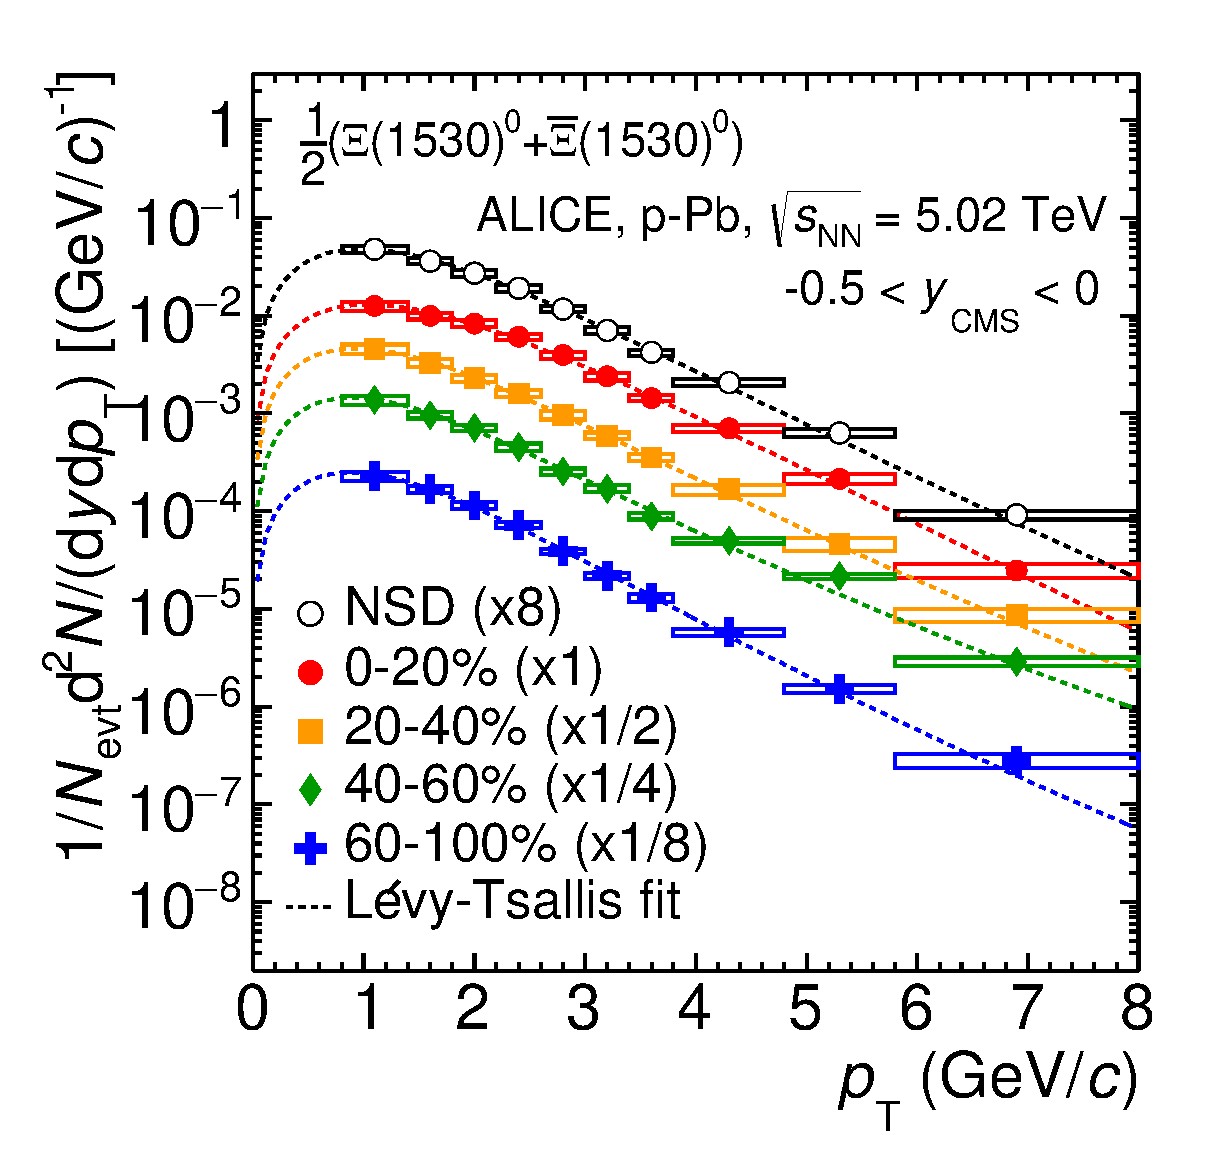
\includegraphics[width=12.0cm]{./Version1/FigChapter5/Spectra/SpectraStatSyspPb.eps}
\caption{Corrected yields as function of \pt~in NSD events and multiplicity dependent event classes in p--Pb collision system. Statistical uncertainties are presented as bar and systematical uncertainties are plotted as boxes.} 
\label{fig:pPb:spectrasysstat}
\end{center}
\end{figure}


\begin{figure}[htbp]
\begin{center}
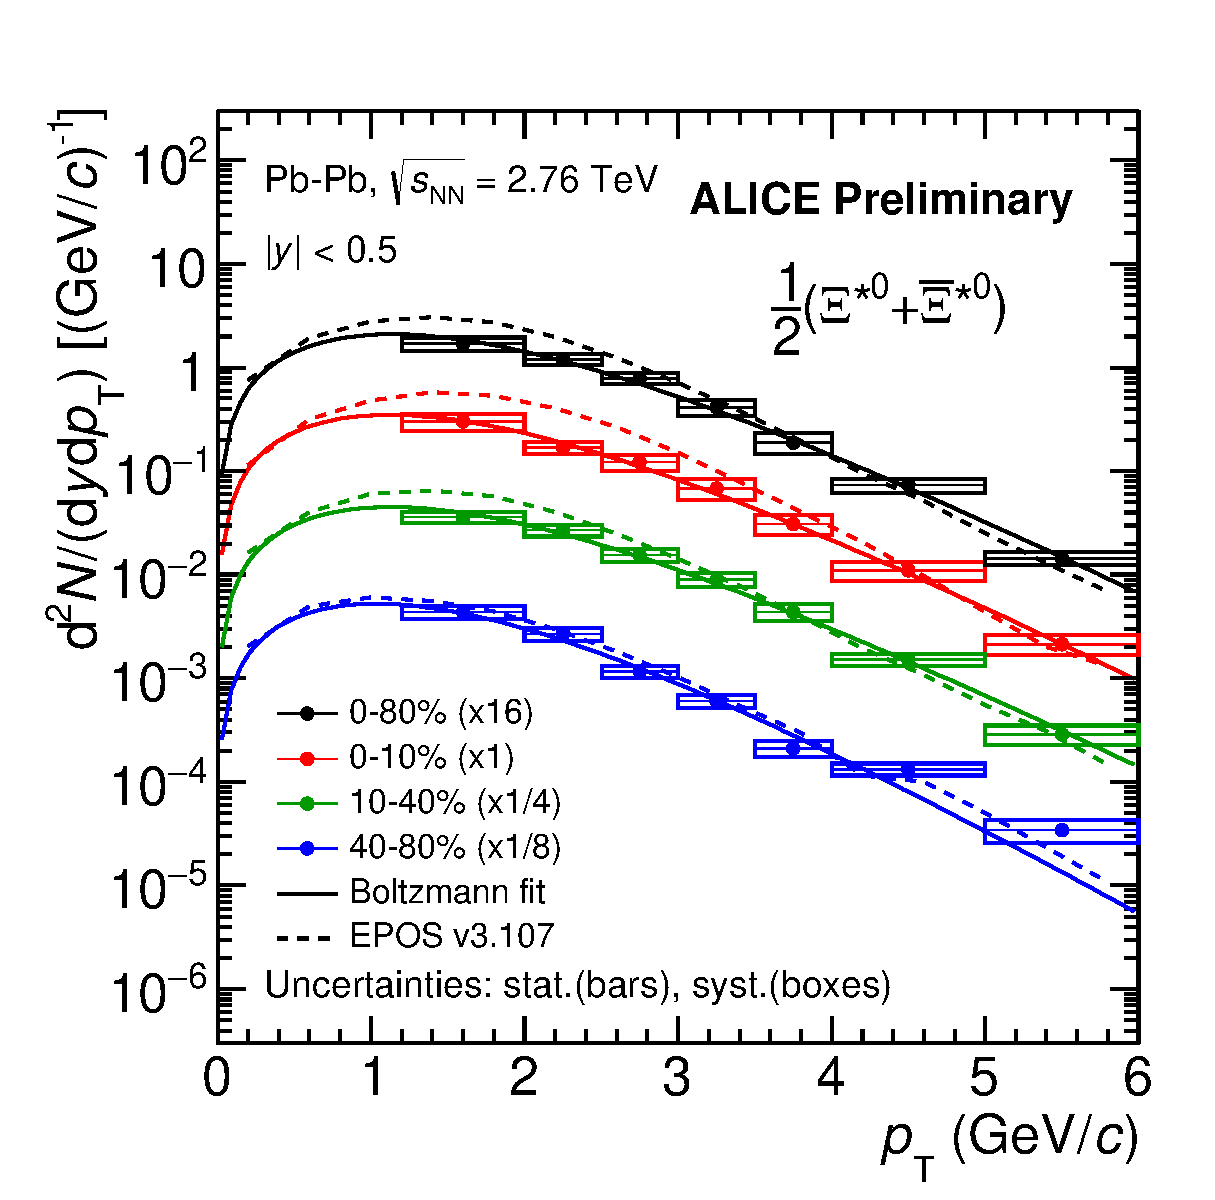
\includegraphics[width=12.0cm]{./Version1/FigChapter5/Spectra/SpectraStatSysPbPb.eps}
\caption{Corrected yields as function of \pt~in different centrality classes in Pb--Pb collision system. Statistical uncertainties are presented as bar and systematical uncertainties are plotted as boxes.} 
\label{fig:PbPb:spectrasysstat}
\end{center}
\end{figure}





